\documentclass[letterpaper,12pt]{article}
\usepackage{tabularx} % extra features for tabular environment
\usepackage{amsmath}  % improve math presentation
\usepackage{amsfonts}
\usepackage{verbatim}
\usepackage{graphicx} % takes care of graphic including machinery
\usepackage[margin=1in,letterpaper]{geometry} % decreases margins
\usepackage{cite} % takes care of citations
\usepackage[final]{hyperref} % adds hyper links inside the generated pdf file

\usepackage{booktabs}

\hypersetup{
	colorlinks=true,       % false: boxed links; true: colored links
	linkcolor=blue,        % color of internal links
	citecolor=blue,        % color of links to bibliography
	filecolor=magenta,     % color of file links
	urlcolor=blue         
}
\usepackage{blindtext}

\usepackage{units}
\usepackage{lineno}
\usepackage{comment}
\usepackage{float}
%++++++++++++++++++++++++++++++++++++++++


\begin{document}
\linenumbers
\title{Uncertain Effects of DFT Functionals on Charge Dynamic of Organic Semiconductor }
\author{authors}
\date{\today}
\maketitle
\begin{abstract}

\end{abstract}

\section{Background}

Theoretical model and computer simulation for understanding a physical system must contain some uncertainties in predicting the system features. 
For example, the theoretical model does not encompass all relevant physical factors, the theoretical model incorporates empirical parameters that include noise, the numerical scheme contains approximation, etc.
Nevertheless, those uncertainties should not affect the validity of the model or the accuracy for the predicting system in terms of some quantities of interest (QoI). 
Here the terminology "uncertainties" refers to the impossibility of getting a deterministic QoI, and excludes theoretical or numerical errors. 

In this work, an investigated model containing uncertainties is the first-principle multiscale model for charge dynamics in organic semiconductors (OSCs).
From a broad perspective, this model contains uncertainties due to the limitation of the model, the randomness nature of the QoI, and the limitation of the numerical simulations.

To explain in detail those uncertainties, the first-principle multiscale model is briefly reviewed. 
Fundamentally, quantum-mechanical description is needed to model charge dynamics due to the motion of electrons. However, the resulting full many-electron schr\"{o}dinger equation is too complex to solve due to complexity, so Density Functional Theory (DFT) appears as a manageable way to model electrons.
DFT has its own challenges in achieving multiscale modeling.

The first challenge relates to the Born-Oppenheimer approximation in quantum
mechanics, which simplifies the problem by separating the electronic and nuclear
coordinates. As a result, the time evolution of the atomic coordinates can be modeled in molecular dynamics (MD) by solving the Newton's equation using empirical force field to approximate the potential energy surfaces (need citation). 

The next challenge is the infeasibility of solving the DFT equations for the entire system even at a fixed time. To address this challenge, state localization is used and the electron's wavefunction becomes localized in space around the nuclei. As a result, the charge dynamic is modeled as a continuous time random walk (CTRW) process, with transition rates between the molecules determined by their electronic structures, namely, the molecule energy, reorganization energy and coupling elements which will be explained in the methodology section. 

In brief summary, the multiscale model can be summarized in Fig. \ref{fig:MSM}.
The process includes: Firstly, classical Molecular Dynamics is used to generate the atomistic coordinates. Then DFT is used to attain electronic structures. Finally the charge dynamic is model as a CTRW among the molecules.

\begin{figure}[h]
    \centering
    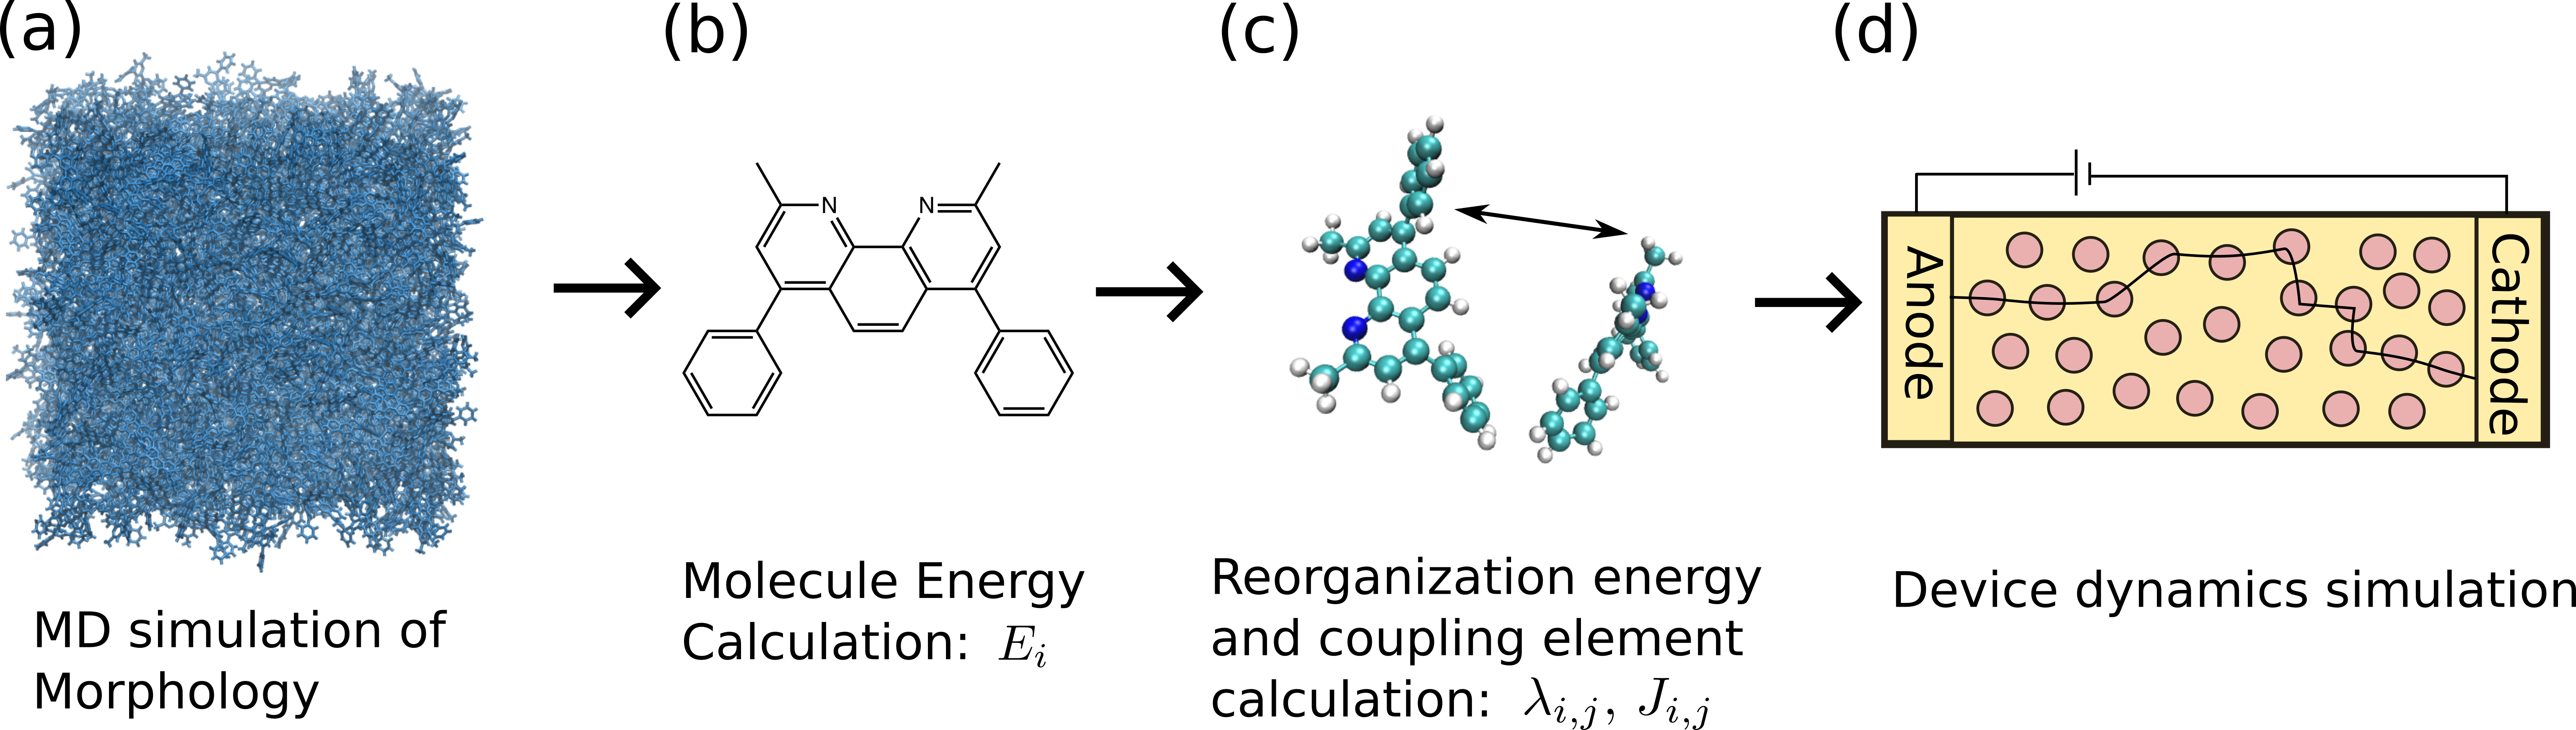
\includegraphics[width=0.95\textwidth]{figs/MSM.png}
    \caption{The multiscale model workflow for OSC. Step 1: MD simulation to generate atom coordinates. Step 2: Molecule energy $E_i$ calculation. Step 3: Calculation of Reorganization energy $\lambda_{ij}$ and coupling element $J_{ij}$ for pairs of molecule $i,j$ whose COM distance is less than $r_\text{cutoff}$. Step 4: Modelling dynamics on device level, such as ToF calculation.}
    \label{fig:MSM}
\end{figure}

In overcoming the challenges and achieving the multiscale model, uncertainties are introduced. 
While Born-Oppenheimer approximation allows for the use of force field to approximate the potential energy surfaces (need citation) and model the atomic coordinates using Newton’s equations, the atomic coordinates are not exactly the same as that modeled by the many-electron schr\"{o}dinger equation.
So the atomic coordinates, that is the molecule structures contain uncertainty which ultimately affects the charge dynamics. 
This is one source of uncertainty that have not been investigated.
But in our investigation, a fixed molecule structure is used and we do not consider this source of uncertainty. 
Secondly, state localization is not exactly a time dependent DFT process. 
But for amorphous OSCs used in this work, model noise from state localization is negligible and we do not consider the uncertainty brought by state localization.
Lastly, the exchange-correlation potential in DFT do not have explicit formula and common practice is to use empirical functional, whose suitability is usually unknown for most molecules.

The charge dynamics is determined by CTRW transition rates, which depend on the electronic structures.
Since DFT is used to calculate the molecular electronic structures, the unknown exchange-correlation functional in DFT will bring uncertainties to the multiscale model. 
In particular, different DFT functionals contain varying levels of Hartree Fock (HF) to represent the exchange-correlation potential. 
The effect of the uncertainty from the DFT exchange-correlation functional on the multiscale model is not yet explored in literatures. 
The goal of this work is to quantify the uncertainty effect of the DFT exchange-correlation functional on the charge dynamics in OSCs and to study the robustness of the multiscale model, with a particular focus on the uncertainty represented by the HF level. 

To perform this goal of uncertainty quantification, a first step is to choose a QoI. A quantity commonly seen in OSC investigation is the charge mobility, which is the distance traveled by the charge carrier divided by the time period. 
The charge mobility is calculated in a \textit{time-of-flight} (ToF) setting. 
As shown in Fig.\ref{fig:MSM}(d), charge carriers are injected into one electrode called \textit{Source} and they are collected by another electrode at the opposite end called \textit{Sink}. 
Knowing the length of the sample $L$ and the time-of-flight $\tau$, the diffusive velocity is calculated as $v_\text{ToF}=\frac{L}{\tau}$.

Most literature report the charge mobility in a steady state setting, where no electrodes are used and the molecular system is infinitely repeated in all three dimensions by periodic boundary conditions. 
Over a long time period, the charge occupation on each molecule $\pi_i$ reach equilibrium, and the steady state diffusive velocity is calculated via:
\begin{equation}
    v_\text{SS} = \sum_i \pi_i \sum_j \omega_{ij} \vec{r}_{ij} = \mathbb{E}f(M_{\infty})
\end{equation} 

Specifically, the focus will be placed on following questions: 
\begin{enumerate}
    \item How does HF level change the electronic structures: reorganization energy, distribution of molecule energies and coupling elements? 
    \item How does HF level change the charge mobility?
    \item Which electronic structure (among energy, coupling element and reorganization energy) uncertainty has the most impact on the charge mobility distribution?
    \item Can we estimate the range of the quantity of interest, given a confidence level?
\end{enumerate}


Calculation of $v_\text{ToF}$ or $v_\text{SS}$ commonly use kinetic Monte Carlo (KMC) to obtain multiple realizations of full charge dynamic trajectories 
or numerically solving the master equation. 
However, those two commonly used methods are not suitable for quantifying the uncertainty effect of multiscale model charge dynamics for the following reasons. 
Firstly, KMC produces random variables whose expectation is the charge mobility. The prior knowledge of the random variable distribution as well as the required KMC samples to achieve converged expectation is unknown. So this method itself pose further challenge for our uncertainty quantification. 
Secondly, the numerical solution of the master equation has stability and convergence issue, that is, a small integration time step is required to achieve stability and a long computational time to achieve convergence result. These aspects add additional difficulty for uncertainty quantification. 
Considering those aspects, the ToF $\tau$ and $v_\text{ToF}$ are obtained via a graph random walk method
\cite{chen_graph_2024}. Once the $v_\text{ToF}$ is calculated using this method, it is considered to be converged. 
Similarly, the steady state occupation $\pi_i$ will be calculated as the null-space of the transition matrix. 

%%%%%%%%%%%%%%%%%%%%%%%%%%%%%%%%%%%%%%%%
\section{Multiscale Model}
The multiscale model results in the charge dynamics becoming CTRW. When there in one charge carrier, each state in CTRW corresponds to the charge occupation in each molecule. The transition rates between the state, that is the rate for charge transfer rates between two molecules $i$ and $j$ is calculated as the Marcus rate:
%
\begin{equation}
    \omega_{ij} = \frac{2\pi}{\hbar} \frac{|J_{ij}|^2}{\sqrt{4\pi R_{ij} k_\text{B}T}} \exp\left(-\frac{(E_{ij} + q \vec{F} \cdot \vec{r}_{ij} - R_{ij})^2}{4R_{ij} k_\text{B}T}\right) ,
    \label{equ:Marcus}
\end{equation}
%
where $\hbar$ is the reduced Planck constant and $k_\text{B}$ the Boltzmann constant. The temperature $T$ (in \unit[]{K}), the charge of the carrier $q$ (in \unit[]{e}) and the external electric field $\vec{F}$ (in V/m) can be considered the external, environmental parameters of the simulation. The vector $\vec{r}_{ij} = (r^x_{ij},r^y_{ij},r^z_{ij})^\text{T}$ connects the center-of-masses (COMs) of molecules $i$ and $j$, which is calculated cyclic boundary conditions depending on the boundary condition. The remaining physical, material-specific (or rather transfer-pair-specific) quantities are the reorganization energy $R_{ij}$, the electronic coupling $J_{ij}$, and the energy difference $E_{ij} = E_i - E_j$ (all in \unit[]{eV}). With the information about the molecular COMs and the rates, one can construct the graph $\mathbf{G}=(\mathbf{V}, \mathbf{W})$ on which the CTRW takes place. $\mathbf{V}$ is a set of nodes (molecules) and $\mathbf{W}: \omega_{ij}$ is the adjacency matrix. A rate is only considered between molecules $i$ and $j$ if their closest-contact distance is smaller than $r_\text{cutoff}=\unit[0.5]{nm}$.

In the section, the components of the multiscale model will be introduced: molecule dynamics, calculation of reorganization energy, molecule energy, coupling element, $v_\text{SS}$ and $v_\text{ToF}$.

%%%%%%%%%%%%%%%%%%%%%%%%%%%%%%%%%%%%%%%%%%%%%%%%%%%%%%%%%
\subsection{Molecule Dynamics Simulation}
In a material system of $N_a$ atoms with mass and position denoted by $m_i$ and $\vec{r}_i$ respectively, molecular dynamics (MD) models the evolution of the atomic coordinate using Newton's second law, which is written in Hamilton equation: 
\begin{equation}
    \begin{cases}
        \frac{d \vec{r}_i}{dt} = \frac{\partial H }{\partial \vec{p}_i} \\
        \frac{d \vec{p}_i}{dt} = -\frac{\partial H }{\partial \vec{r}_i}
    \end{cases}
    \label{eq:Hamilton}
\end{equation}
for $i=1,\cdots,N_a$, where the Hamiltonian $H$ reads:
\begin{equation}
    H=\sum\limits_{i} \frac{|\vec{p}_i|^2}{2 m_i} + U(\vec{r}_1,\cdots,\vec{r}_{N_a})
    \label{eq:Hamilton2}
\end{equation} 

In principle the potential energy function $U(\vec{r}_1,\cdots,\vec{r}_{N_a})$ of the system can be obtained from electronic structure models. In practice, it is a very computationally expensive procedure, and without too much loss in precision, MD use empirical potentials that are designed for specific purposes.
In our work, constant the molecule number $N=1000$, a temperature $T=300$ K and a pressure at 1 atm is used to achieve an NPT ensemble. 
One of the final BCP morphology is chosen as OSC for charge transport study. 

%%%%%%%%%%%%%%%%%%%%%%%%%%%%%%%%%%%%%%%%%%%%%%%%%%%%%%%%%%
\subsection{Electronic Structure Calculations} 
%Each molecule is an $N_\text{el}$-electron system, and in quantum mechanics, the probability of finding electrons in space is described by the electron wavefunction $\phi(\vec{r})$.
Effective single-electronic wave functions $\phi_l (\vec{r})$ and associated energies $\epsilon_l$ for a system with $N_\text{el}$ electrons are determined as solutions to the Kohn--Sham equations~\cite{kohn_self_1965}
%
\begin{equation}
    \left(-\frac{1}{2}\nabla^2_{\vec{r}} + v_\text{ext}(\vec{r}) + v_\text{H}[\rho](\vec{r}) + v_\text{XC}[\rho](\vec{r})\right) \phi_l(\vec{r}) =  \epsilon_l \phi_l (\vec{r}) ,
    \label{eq:KS2}
\end{equation}
%
where $v_\text{ext}$ in an external potential (typically from the nuclei), $v_\text{H}[\rho]$ the electrostatic Hartree potential of a classical charge density $\rho(\vec{r})$, and $v_{XC}[\rho]$ the exchange-correlation functional containing explicit quantum-mechanical electron-electron interactions. The charge density is determined from the single-particle wave functions as $\rho(\vec{r})=\sum\limits_{l=1}^{N_\text{el}} \left\vert\phi_l(\vec{r})\right\vert^2$. 
 

%
\begin{equation}
    U[\rho] = T_s[\rho] + \int \hat{V}_\text{ext}(\vec{r}) \rho(\vec{r}) d \vec{r} + \hat{V}_\text{H}[\rho] + \hat{V}_\text{XC}[\rho]
    \label{eq:KS_model}
\end{equation}
%
where the electron density is , $T_s[\rho]$ is the kinetic energy depending on $\rho$,  $\hat{V}_\text{ext}$ is the external potential energy,  $\hat{V}_\text{H}[\rho]$ is the Hartree energy accounting for the Coulomb interaction, $\hat{V}_\text{XC}[\rho]$ is the exchange-correlation energy accounting for the difference between classical and quantum effect. The exact form of $\hat{V}_\text{XC}[\rho]$ is not known, in practice, this energy term is approximated by DFT functionals. In our work, different functionals are tested on BCP molecular system to check the effect of different functionals' impact on charge mobility. Different functionals have different ways to represent the exchange-correlation potentials, such as different level of HF exchange potential. 
Then PBE0 functional is used with varying HF component in the exchange-correlation potentials. 

In practice, Equation \ref{eq:KS2} is solved iteratively, and the wave function is represented by a linear combination of basis functions call basic sets. 
In this work, the basic set def2-tzvp \cite{weigend_accurate_2006} is used. The DFT computation is performed by VOTCA \cite{Baumeier2011} which internally calls ORCA software.


The internal energy $U_i$ of molecule $i$ depends on the charge states and atomic coordinate (also called geometry) of the molecule. 
The optimized geometry of a molecule refers to the atomic coordinates that minimize $U_i$.
Here we use $U_i^\text{xX}$ to denote the internal energy of molecule $i$ at charge state x in the optimized geometry X. Neutral and charge states are represented as x=n and c, respectively. Similarly, optimized neutral molecular geometry and optimized charge molecular geometry are represented by X=N and C, respectively.

The reorganization energy $R_{ij}$ from molecule $i$ to molecule $j$ is given as:
\begin{equation}
    R_{ij} = U_i^\text{nC} - U_i^\text{nN} + U_j^\text{cN} - U_j^\text{cC}
\end{equation}
where $U_i^\text{nC}$ is the internal energy of the neutral molecule $i$ in optimized geometry of charged molecule, calculated from Equation \ref{eq:KS_model}. 
And $U_i^\text{nN}$ the internal energy of the neutral molecule $i$ in optimized geometry of neutral molecule. Similarly, $U_j^\text{cN}, U_j^\text{cC}$ are defined in this way.
When charge carriers are holes, a charged molecule has one electron less compared to a neutral molecule. 
For the BCP device, we obtain $R_{ij}=0.50$ eV since this is only one type of molecule.

In a single-component system where internal energy difference of molecule $i$ and $j$ is equal, the energy difference $E_{ij}$ is calculated by:
\begin{equation}
    E_{ij} = E_i - E_j
    \label{eq:siteE}
\end{equation}
where $E_i = E_i^\text{c} - E_i^\text{n},E_j = E_j^\text{c} - E_j^\text{n}$ are the molecule energies, the superscript represents charge state or neutral state molecule as mentioned above. And $E_i^\text{n} = E_i^\text{n,el} + E_i^\text{n,induce}$ considers the electrostatic energy as well as the energy from the induced dipole moment.
In multiscale model, $E_i^\text{n} = E_i^\text{n,el} + E_i^\text{n,induce}$ is calculated iteratively from the Thole Model as detailed in \cite{thole_molecular_1981}.
% instead of using a dielectric constant as been done in the bulk system at macroscopic scale. 
Specifically, the first step is to calculate the induced dipole at atom $a_i$ by electrostatic field. This induced dipole will change the dipole moment at all other atoms $b_j \neq a_i$. Then repeat this step and recalculate the induced dipole at atom $a_i$, followed by induced dipoles at all other atoms $b_j$. This process is repeated until the induced dipole converge to a fix value. 
In short summary, the $E_i$ is a function of all individual atoms' charges $q$ and induced dipole $\mu$: $E_i^\text{n,el} + E_i^\text{n,induce} = \sum\limits_{a_i} f(q_{a_i}, \mu_{a_i})$ where $a_i$ goes over all the atoms in the system. 
The calculation of $E_i^\text{c} = E_i^\text{c,el} + E_i^\text{c,induce}$ uses similar iteratively process as $E_i^\text{n}$.
The molecule energies and their distribution are shown in the appendix.

%%%%%%%
The coupling element $J_{ij}$ between molecule $i$ and $j$ is calculated \cite{baumeier_density_2010} using the electron wave function of the molecules obtained from the Kohn-Sham equation: 
\begin{equation}
    J_{ij} = \frac{ J^0_{ij}- \frac{1}{2}(e_i+e_j) S_{ij} }{ 1- S_{ij}^2 }
    \label{equ:JAB}
\end{equation}
where $J^0_{ij} = \langle \phi^\text{HOMO}_i | \hat{H} | \phi^\text{HOMO}_j \rangle $, $e_i = \langle \phi^\text{HOMO}_i | \hat{H} | \phi^\text{HOMO}_i \rangle $, $e_j = \langle \phi^\text{HOMO}_j | \hat{H} | \phi^\text{HOMO}_j \rangle $, and $S_{ij}=\langle \phi^\text{HOMO}_i | \phi^\text{HOMO}_j \rangle $ with bra-ket notation.
For hole-transporting OSCs system such as the BCP used in this work, $\phi^\text{HOMO}_i$ is the HOMO electron wave function of molecule $i$. 
The Kohn-Sham Hamiltonian is $\hat{H} = -\frac{1}{2}\nabla^2_{\vec{r}} + \hat{V}_\text{ext} + \hat{V}_\text{H}[\rho] + \hat{V}_\text{XC}[\rho]$. 
A single molecule is called a monomer, and a pair of two molecules is called a dimer.

Denote $\phi^\text{HOMO}_\text{D}$ as the HOMO electron wave function of the dimer,  $J^0_{ij}$ can be calculated via:
$
    J^0_{ij} = \mathbf{p}^i \text{diag}(\mathcal{E}) \mathbf{p}^j
$, 
where the vector $\mathbf{p}^i = \langle \phi_i^\text{HOMO} | \phi^\text{HOMO}_\text{D} \rangle$ and $\mathbf{p}^j = \langle \phi_j^\text{HOMO} | \phi_\text{D}^\text{HOMO} \rangle$ are called the projections of the monomer orbitals $\phi_i^\text{HOMO}, \phi_j^\text{HOMO}$ onto the dimer orbitals $\phi^\text{HOMO}_\text{D}$. And $\text{diag}(\mathcal{E})$ is the diagonal matrix consisting eigenvalues of the basis function of $\phi_\text{D}^\text{HOMO}$. The molecular coupling element distribution is shown in the appendix.

%%%%%%%%%%%%%%%%%%%%%%%%%%%%%%%%%%%%%%%%%%%%%%%%%%%%%%%%%%%%%%%%%%

\section{Time-of-flight Calculation}
The multiscale model defines a graph $\mathbf{G}$ with an adjacency matrix $\mathbf{W}$, where the nodes represent molecules and the edge weights $\omega_{ij}$ represent the Marcus rate from molecule $i$ to molecule $j$. 
The charge dynamics are modeled as a continuous-time random walk on this graph. In the time-of-flight (ToF) model, some vertices serve as \textit{Source} nodes, representing the electrode where charge carriers are injected, and some as \textit{Sink} nodes, where charge carriers are detected and the ToF is recorded.

In CTRW the ToF is calculated as the expected hitting time of a continuous time Markov chain.

For a system with $N$ molecules and one charge carriers, there are $N$ possible occupation states. A state is called the Source state if one of the Source molecule is occupied, and a Sink state is the one when one of the Sink molecule is occupied.

The transition rates between the states defines the adjacency matrix $\mathbf{W}:\omega_{ij}$.
According to such connectivity between the molecules, the transition rates $\mathbf{W}_{ij}$ from state $i$ to $j$ is:
\begin{equation}\label{eq:transition_rates}
	\mathbf{W}_{ij} =
	\begin{cases}
	     0			&  i \text{ is not connected to } j,\\
         \omega_{ij}   &  i \text{ is connected to } j,
	\end{cases}
\end{equation}

Then the transition probability from state $i$ to $j$ is $p_{ij} = \mathbf{W}_{ij}/D_i$ where $D_i := \sum_{j} \mathbf{W}_{ij}$.
And the expected time from state $i$ to reach the Sink state $\tau_i$ is calculated via: 
\begin{equation}\label{eq:hitting_time}
	\tau_i = \begin{cases}
		\frac{1}{D_i} + \sum_{j \ne i} p_{ij} \tau_{j} &\text{if $i$ is not a sink state},\\
		0 &\text{else.} 
	\end{cases}
\end{equation} 

To account for all possible starting nodes of the carriers, all Source states must be considered. The random walk process can be modeled as a parallel electric network of capacitors \cite{doyle_random_2000}. Accordingly, the ToF is evaluated using the harmonic mean:
\begin{equation} 
\tau = N_\text{source} \left[\sum_{i \in \text{Source}} (\tau_i)^{-1}\right]^{-1},
\label{eq:ToF}
\end{equation}
where $N_\text{source}$ is the number of Source states.

To calculate $v_\text{SS}$ the steady state distribution $\pi_i$ is required. In continuous time Markov chain, the steady state distribution vector $\vec{\pi}: \pi_i$ is the null-space of $\mathbf{W}-\mathbf{D}$:
\begin{equation}
    (\mathbf{W}-\mathbf{D} )\vec{\pi} = \mathbf{0}
\end{equation}
where $\mathbf{D} = \text{diag}(D_i)$ is the out-degree matrix of $\mathbf{W}$.
%%%%%%%%%%%%%%%%%%%%%%%%%%%%%%%%%%%%%%%%%%%%%%%%%%%%%%%%%%

\section{Results on MADN}

In this study, we investigate the hole-transporting organic semiconductor MADN (2-Methyl-9,10-di(naphth-2-yl)anthracene). Essential steps in our multiscale model involve calculating the dipole moment $\mu$ and the isotropic polarizability $P_\text{iso}$ for both neutral and charged states in the optimized geometry MADN molecule. These properties are crucial for evaluating molecular energy contributions from electrostatic and polarization effects.

Figure \ref{fig:autogen_MADN} illustrates the dependence of the dipole moment $\mu$, isotropic polarizability $P_\text{iso}$, reorganization energy $\lambda$, and energy disorder $\sigma(E)$ on the Hartree-Fock exchange (HFX) parameter.

%
\begin{figure}[H]
    \centering
    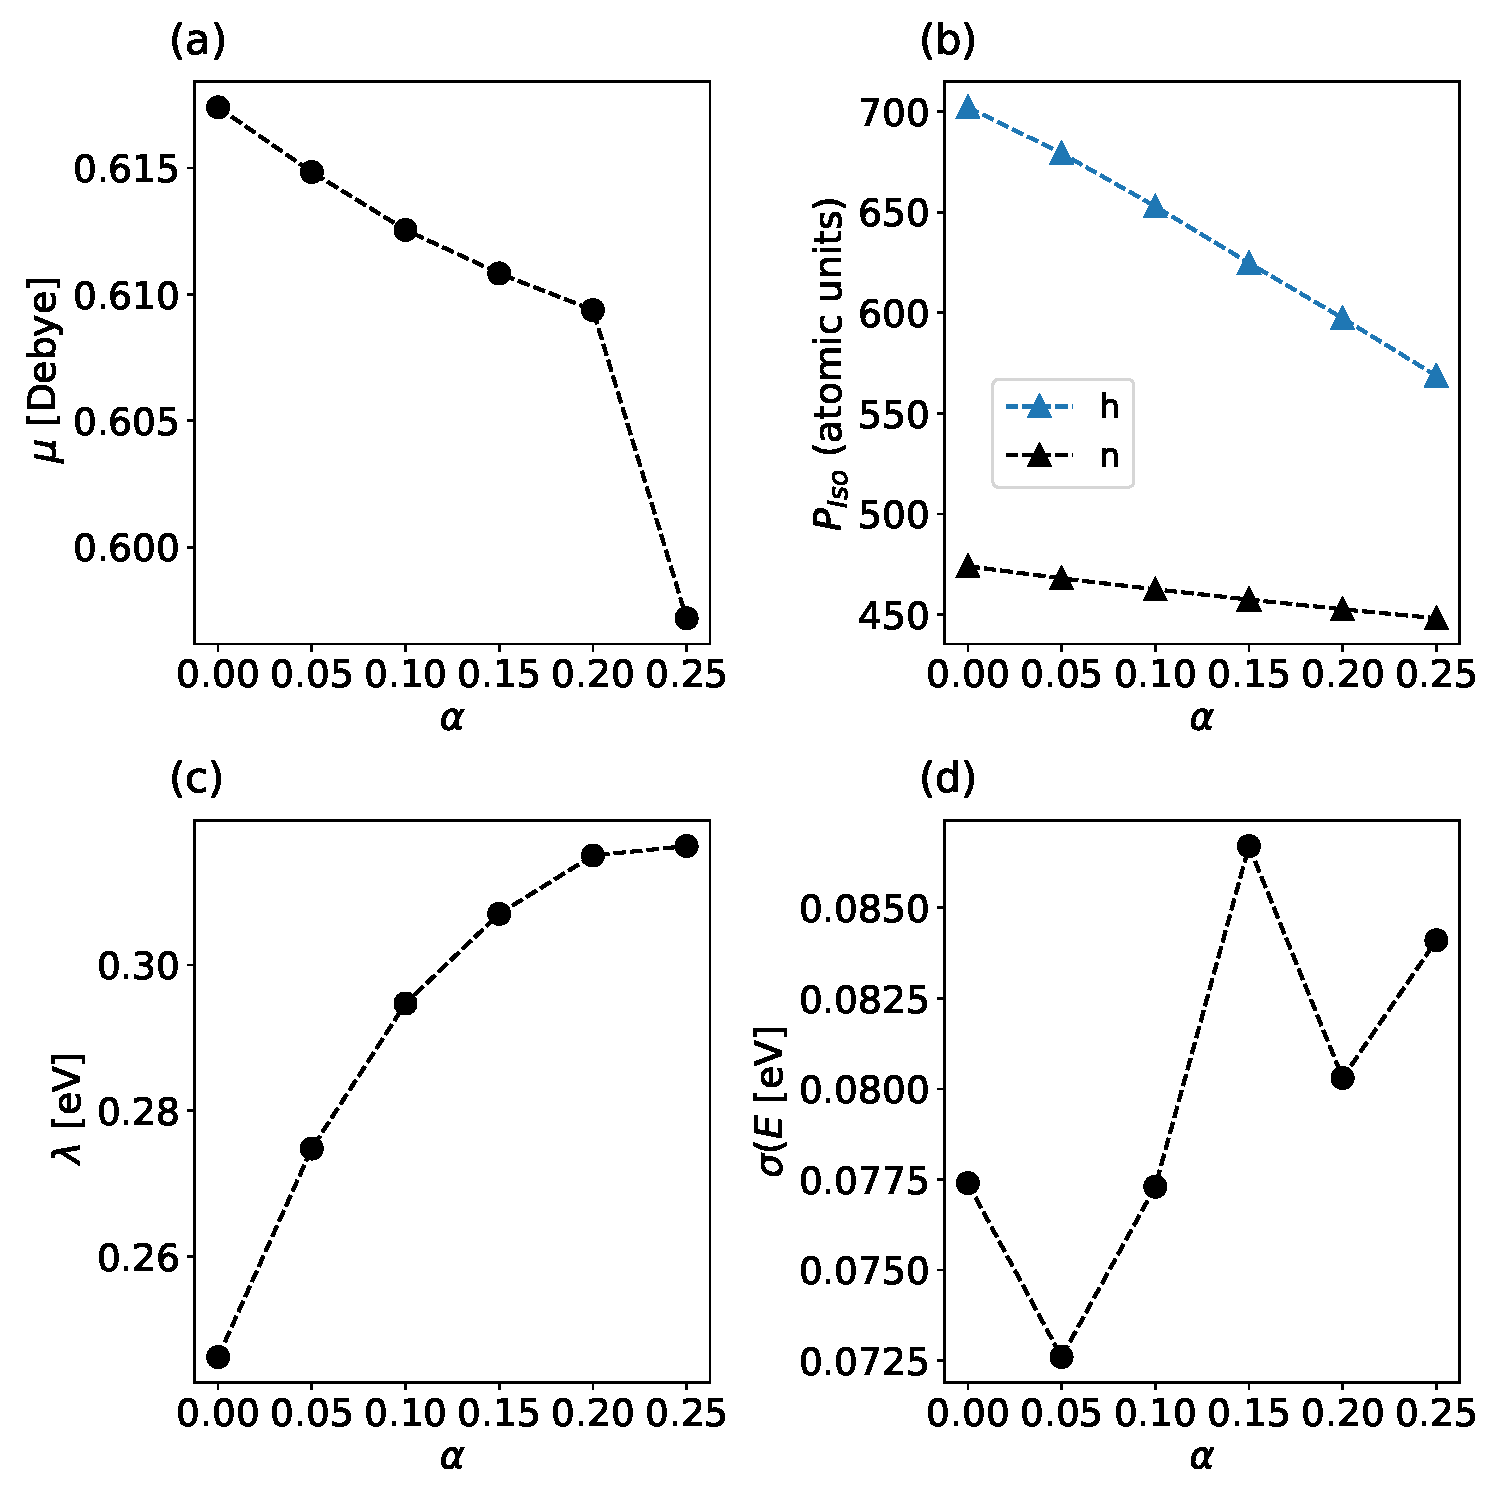
\includegraphics[width=0.80\textwidth]{figs/MADN_HFX/fig_autogen.pdf}
    \caption{(a) The dipole moment of neutral state MAND molecule $\mu$, (b) isotropic polarizability $P_\text{iso}$, (c) reorganization energies $\lambda$ and (d) energy disorder $\sigma(E)$ as a function of the HFX parameters (denoted by $\alpha$).}
    \label{fig:autogen_MADN}
\end{figure}
% 


Figure \ref{fig:autogen_MADN}(a) shows a decrease in the dipole moment with increasing HFX, exhibiting a notable drop at HFX = 0.25. 

Figure \ref{fig:autogen_MADN}(b) demonstrates a linear decrease in isotropic polarizability for both neutral and charged MADN states as HFX increases from 0 to 0.25, indicating reduced molecular polarizability.

Figure \ref{fig:autogen_MADN}(c) indicates an increase in reorganization energy $\lambda$ with higher HFX, reflecting greater energy requirements for electronic adjustments during charge transfer. This increase is nonlinear compared to the linear decrease in $P_\text{iso}$.

Figure \ref{fig:autogen_MADN}(d) shows that the energy disorder $\sigma(E)$ for MADN are similar and close to \unit[0.08]{eV} under different HFX values.

The ToF and corresponding diffusive velocity $v_\text{ToF}$ are presented in Table \ref{tab:ToF_MADN_HFX}. For boundary conditions, the \textit{Source} region contains molecules with X-coordinates $0 < r^x_i < 0.5$ nm, and the \textit{Sink} region contains molecules with X-coordinates $8.5 < r^x_i < 9$ nm. We also consider scenarios without energy disorder to model systems where all molecules have uniform energy.

\begin{table}[H]
    \centering
    \begin{tabular}{c c c c c}
    \hline
        $\alpha$ & ToF [s] & $v_\text{ToF}$ [m/s] & ToF(no $E$) [s] & $v_\text{ToF}$ (no $E$) [m/s] \\
    \hline
        0.00 &  $6.4 \times 10^{-9}$ & 1.2 & $1.9 \times 10^{-10}$ & 42 \\
        0.05 & $ 7.9 \times 10^{-9}$ & 1.0 & $4.1 \times 10^{-10}$ & 20 \\
        0.10 & $ 1.6 \times 10^{-8}$ & 0.51 & $4.0 \times 10^{-10} $ & 20 \\
        0.15 & $ 3.0 \times 10^{-8}$ & 0.31 & $4.0 \times 10^{-10} $ & 25 \\
        0.20 & $ 2.1 \times 10^{-8}$ & 0.39 & $4.5 \times 10^{-10}$ & 18 \\
        0.25 & $ 9.5 \times 10^{-8}$ & 0.083 & $7.2 \times 10^{-10}$ & 11 \\
    \hline
    \end{tabular}
    \caption{The ToF and diffusive velocity calculated by ToF along a distance $L_x = 8$ [nm] with and without energy disorder of the MADN system as a function of the HFX. }
    \label{tab:ToF_MADN_HFX}
\end{table}

Table \ref{tab:ToF_MADN_HFX} shows that as HFX increases from 0 to 0.25, the ToF with energy disorder increases by a factor of approximately 15, while without energy disorder, the increase factor is about 4. This increase in ToF is attributed to the rise in $\lambda$, changes in molecular energies, and variations in coupling elements.

Figure \ref{fig:E_qmmm_MADN} presents a scatter plot comparing the site energies of MADN molecules across different HFX values, using HFX = 0.25 (PBE0 functional) as a reference. The energies consistently fall within the range of -0.5 to -1.1 eV, with data points clustering near the diagonal line, indicating similar molecular energies regardless of HFX variation.

\begin{figure}[H]
    \centering
    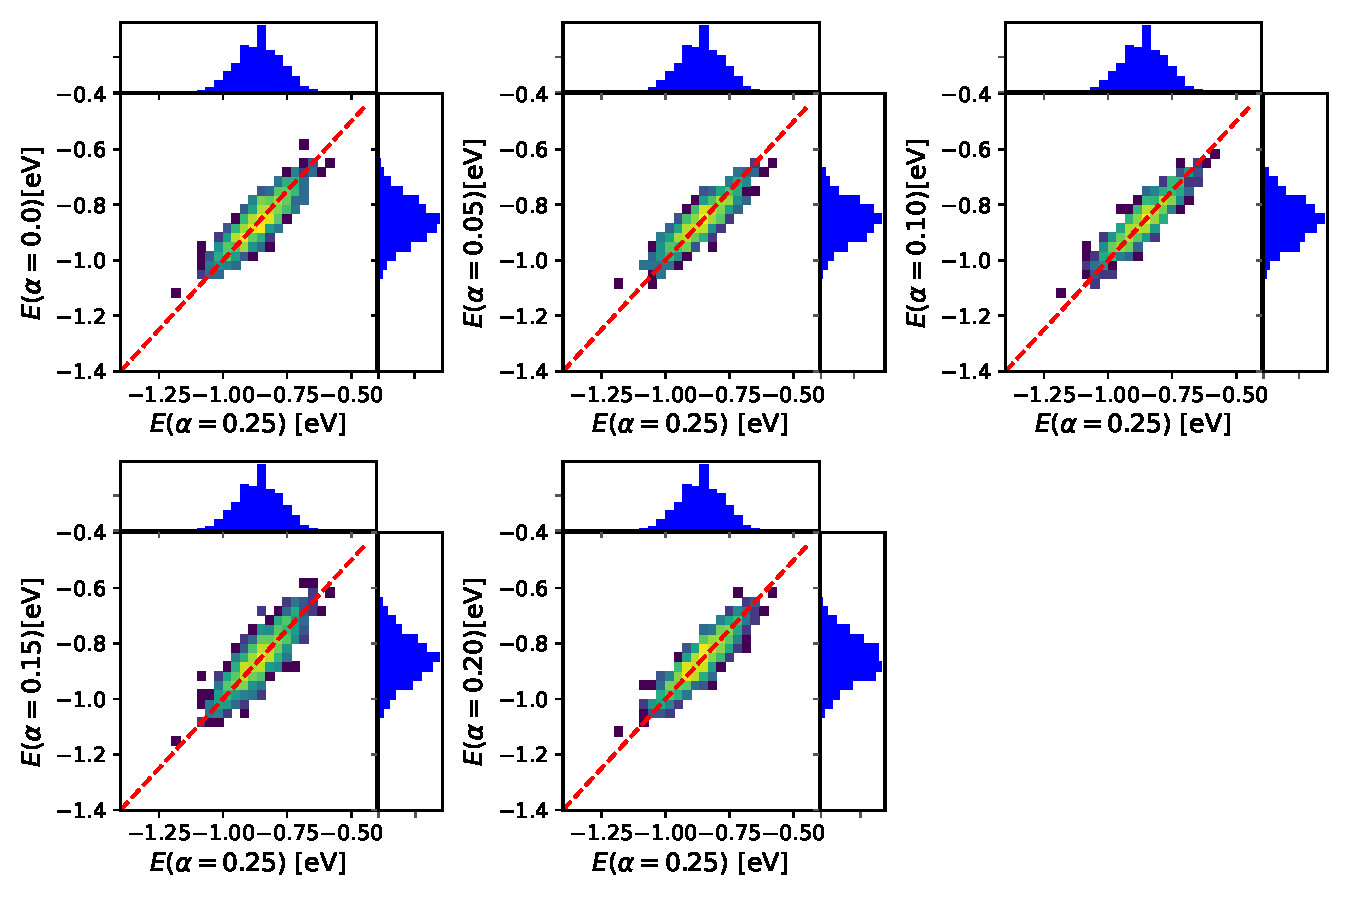
\includegraphics[width=0.95\textwidth]{figs/MADN_HFX/scatterE_qmmm.pdf}
    \caption{Scatter plot of site energy of MADN molecules calculated from different HFX, compared to the site energy calculated from HFX=0.25 (The PBE0 functional). The brighter color near the diagonal lines indicates denser population of the molecules.  The top and right histogram show the energy distributions.}
    \label{fig:E_qmmm_MADN}
\end{figure}


Figures \ref{fig:Estat_qmmm_MADN} and \ref{fig:Edip_qmmm_MADN} show that both electrostatic and polarization energies remain consistent across HFX values from 0 to 0.25, further clustering near the diagonal.


\begin{figure}[H]
    \centering
    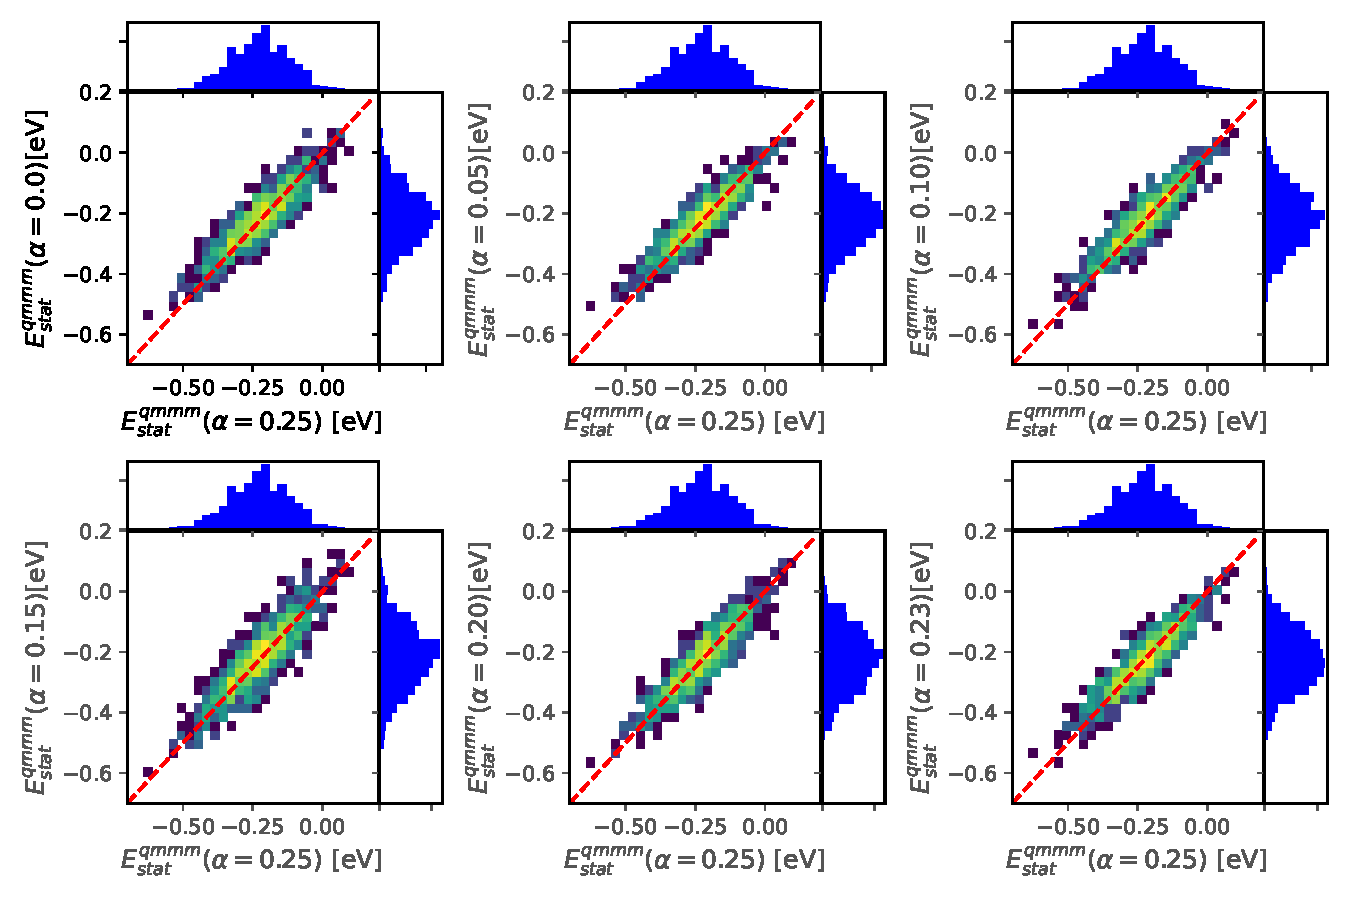
\includegraphics[width=0.95\textwidth]{figs/MADN_HFX/scatterEstat_qmmm.pdf}
    \caption{Scatter plot of MADN electrostatic energy calculated from different HFX, compared to the electrostatic energy calculated from HFX=0.25 (The PBE0 functional). The brighter color near the diagonal lines indicates denser population of the molecules.  The top and right histogram show the energy distributions.}
    \label{fig:Estat_qmmm_MADN}
\end{figure}

\begin{figure}[H]
    \centering
    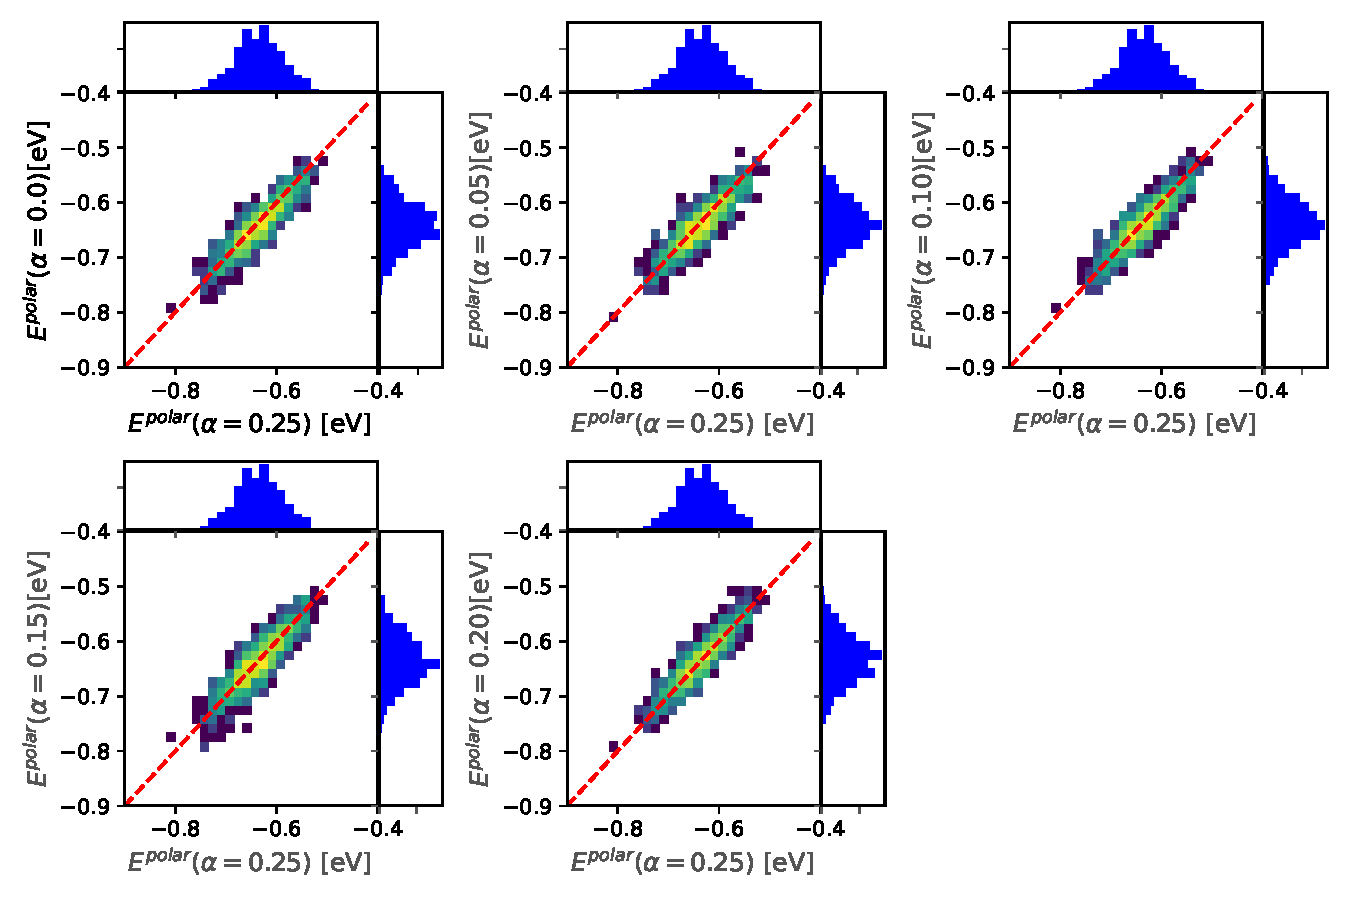
\includegraphics[width=0.95\textwidth]{figs/MADN_HFX/scatterEdip_qmmm.pdf}
    \caption{Scatter plot of MADN polarization energy calculated from different HFX, compared to the polarization energy calculated from HFX=0.25 (The PBE0 functional). The brighter color near the diagonal lines indicates denser population of the molecules.  The top and right histogram show the energy distributions.}
    \label{fig:Edip_qmmm_MADN}
\end{figure}

The electrostatic energy ranges from 0.1 to -0.6 eV, while polarization energy spans -0.5 to -0.8 eV.  Similar to the molecule energy, the data points are clustered near the diagonal line. 
The standard deviations of the electrostatic energy are 0.099, 0.094, 0.099, 0.11, 0.10, \unit[0.10]{eV}, and the standard deviations of the polarization energies are 0.044, 0.043, 0.043, 0.047, 0.045, \unit[0.045]{eV}. So the disorder in electrostatic energies is consistently larger than than in molecule energies, and the palorization effect reduces the electrostatic energy disorder. 
Each individual molecule has similar polarization energies under different HFX calculation, in spite of $P_\text{iso}$ is linearly dependent on HFX. 

The coupling element obtained with different HFX for each molecular pair compared to that obtained with HFX=0.25 is shown in the scatter plot Fig. \ref{fig:J_MADN}.
\begin{figure}[H]
    \centering
    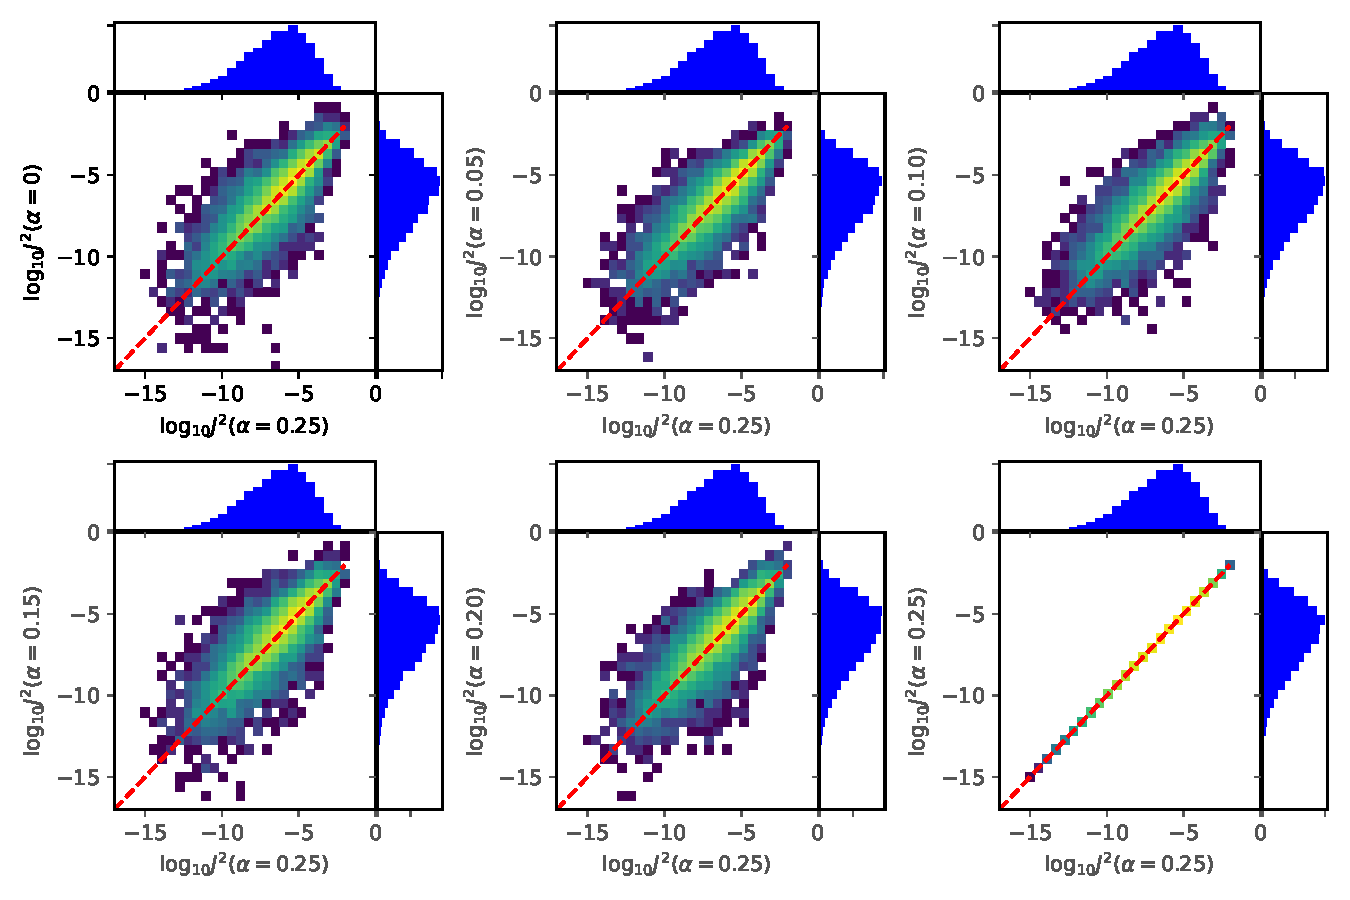
\includegraphics[width=0.95\textwidth]{figs/MADN_HFX/scatterJ_all.pdf}
    \caption{Scatter plot of MADN coupling element $\log_{10} J^2$ calculated from different HFX, compared to the polarization energy calculated from HFX=0.25 (The PBE0 functional). The brighter color near the diagonal lines indicates denser population of the molecules.  The top and right histogram show the energy distributions.}
    \label{fig:J_MADN}
\end{figure}

The distribution of $\log_{10} J^2$ has a range of -14 to -2, and for all HFX values, the distribution has a peak at around -5. 
For large values $\log_{10} J^2 < -5$ the coupling element remains consistent across HFX values from 0 to 0.25, while for large values $\log_{10} J^2 > -5$, the calculated coupling elements for a specific molecular pair can have large variation due to HFX values. 

In charge transport network, $J^2$ undirectional for a molecular pair, and decays exponentially as the mutual center-of-mass distance increases. The large $\log_{10} J^2$ are usually observed for molecular pairs with small center-of-mass distance. And the charge dynamics is more dominated by those large $\log_{10} J^2$ compared to the small $\log_{10} J^2$. 

To determine the range of $\log_{10} J^2$ that are significant for the charge dynamics, a percolation algorithm is performed with procedure as:
\begin{enumerate}
    \item A critical value $J_c$ is chosen,
    \item In graph $\mathbf{G}$ remove all the edges with $J^2 < J_c^2$
    \item Calculate the maximum size $\max({N_\text{sub}})$ of the connected subgraphs
\end{enumerate}

\begin{figure}[H]
    \centering
    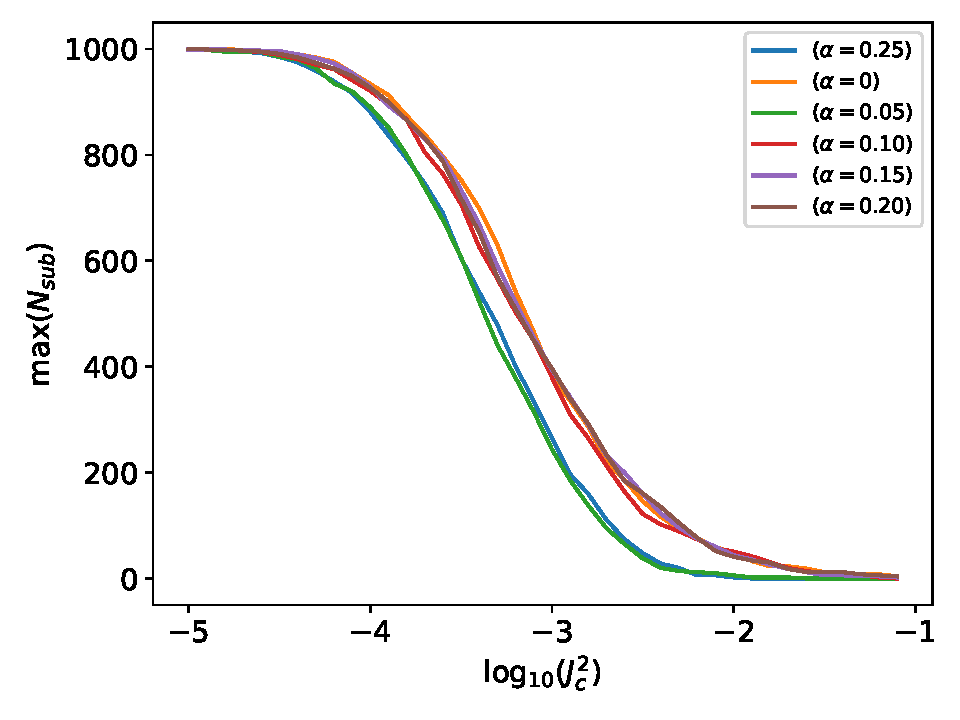
\includegraphics[width=0.75\textwidth]{figs/MADN_HFX/fig_network_all.pdf}
    \caption{The maximum size of the subgraphs obtained in the percolation algorithm as a function of critical value $J_c$. The molecular systems obtained by different HFX are colored according to the legend.}
    \label{fig:J_percolate}
\end{figure}
Figure \ref{fig:J_percolate} shows the dependence of $\max({N_\text{sub}})$ on the critical value $J_c$. When $\log_{10} J_c^2 < -4.5$, $\max({N_\text{sub}})$ is 1000, meaning that removing all the edges with $J^2 < 3.1 \times 10^{-5}$ the 1000 vertexes still form a connected graph. 
But when removing the edges with $J^2 < 3.1 \times 10^{-4}$ ( corresponding to $J_c > -3.5$), the maximum size subgraph is 600, and it quickly decreases as $J_c$ increases, showing a phase transition. 
So the dominated coupling elements are those with $\log_{10} J_c^2 > -4.5$. 
And the variation in small $J$ due to HFX has less impact on the charge dynamics. 

In this section we answer the question of how does HF level change the electronic structures and 
how does HF level change the charge mobility. 
In the next section, uncertainty quantification via Monte Carlo method and sensitivity analysis is perform to answer which electronic structure (among energy, coupling element and reorganization energy) uncertainty has the most impact on the charge mobility distribution. 
And further estimate the range of the quantity of interest, given a confidence level.
%%%%%%%%%%%%%%%%%%%%%%%%%%%%%%%%%%%%%%%%%%%%%%%%%%%%%%%%%

\section{ToF Distribution and Sensitivity Analysis}
The previous section shows that different HFX affect the calculated ToF. In this section, we use the Monte Carlo method to estimate the range of the ToF given a confidence level, followed by a sensitivity analysis to determine which parameter contributes more to the variance of ToF. 

\subsection{ToF Distribution}
The ToF is calculated from electronic structure ($E$, $\lambda$ and $\log_{10}(J^2)$) data, that is, ToF is a function with the input of all electronic structure parameters:
\begin{equation}
    \tau = g(x_1,x_2,\cdots, x_N) \; 
\end{equation}
where the parameters $(x_1,x_2,\cdots, x_N)$ represents $(E_i, J_{ij}, \lambda)$ for all $i,j=1,2,\cdots,N$ and $J_{ij}>0$. 

Since the exchange-correlation functional is not known and each molecule has a slightly different structure compared to the optimized structure, each parameter $(x_1,x_2,\cdots, x_N)$ has uncertain. 
To estimate the uncertainty, we consider the maximum amount of uncertainties according to the obtained $(E_i, J_{ij}, \lambda)$ with the six different HFX.
To achieve this, each parameter can be modeled as a normal distribution with the mean and standard deviation being the HFX sample mean and standard deviation, respectively.

Then Monte Carlo scheme is used to estimate the distribution of the ToF. The Monte Carlo scheme has the procedure:
\begin{enumerate}
\item For all $i=1,2,\cdots, N$, sample a realization $(x_1,x_2,\cdots, x_N)$ where each parameter $x_i \in (x_1,x_2,\cdots, x_N)$ has the normal distribution $x_i \in \mathcal{N}(\bar{x}_i, \sigma_{x_i})$. 
\item Calculate ToF using the sampled data set $(x_1,x_2,\cdots, x_N)$. 
\item Repeat step 1 and 2 for $N_\text{MC} = 50000$ times to obtain ToFs. Plot the distribution of the ToFs.
\item Fit the distribution of $log_{10}(\text{ToF})$ to Gamma distribution.
\end{enumerate}

The distribution of ToF calculated as the CTMC where transition parameters are varied is unknown, so we attempt to fit the distribution of ToF to Gamma distribution. The reason is as followed.

From equation \ref{eq:hitting_time}, the ToF can be considered as the some combination of occupation time in the molecules, which is $log_{10}(\omega_{i}^{-1})$. 
When the parameters $E, J_{ij}, \lambda_{ij}$ are normally distributed random variables, the calculated ToF shows that variables $E,\lambda_{ij}$ has a larger influence than $J_{ij}$. 
The Marcus rate uses $E,\lambda_{ij}$ in the exponential form. If $\Delta E$ is normally distributed, then $log_{10}(\omega_{i}^{-1})$ is Gamma distributed. 
Since $E$ has greater influence to ToF than $\lambda_{ij}, J_{ij}$ and to be consistent, Gamma distribution is used to fit the Monte Carlo sampled ToF in all the investigated cases.

To understand which uncertainty among $E, \lambda, J_{ij}$ has a greater impact on the ToF, we study the following distribution of ToF:
\begin{enumerate}
    \item Fixed the $\lambda$ to be the averaged $\bar{\lambda}$, and $J_{ij}$ to be the averaged $\bar{J}_{ij}$. Then each molecule energy $E_i$ is sampled from the normal distribution $\mathcal{N}(\bar{E}_i, \sigma^2_{E_i})$. Finally obtain and plot $N_\text{MC}$ sample of $\tau$, whose distribution is denoted as $P(\log_{10}(\tau)|E_i \text{ uncertain})$.
    \item Fixed the $E_i$ to be the average $\bar{E}_i$ and and $J_{ij}$ to be the averaged $\bar{J}_{ij}$. Then $\lambda$ is sampled from the normal distribution $\mathcal{N}(\bar{\lambda}, \sigma^2_{\lambda})$. Finally obtain and plot $N_\text{MC}$ sample of $\tau$, whose distribution is denoted as $P(\log_{10}(\tau)|\lambda \text{ uncertain})$. 
    \item Fixed the $E_i$ to be the average $\bar{E}_i$ and $\lambda$ to be the averaged $\bar{\lambda}$. Then $J_{ij}$ is sampled from the normal distribution $\mathcal{N}(\bar{J}_{ij}, \sigma^2_{J_{ij}})$. Finally obtain and plot $N_\text{MC}$ sample of $\tau$, whose distribution is denoted as $P(\log_{10}(\tau)|J_{ij} \text{ uncertain})$.
    \item Both $E_i$, $\lambda$ and $J_{ij}$ are sample from their normal distribution: $\mathcal{N}(\bar{E}_i, \sigma^2_{E_i})$, $\mathcal{N}(\bar{\lambda}, \sigma^2_{\lambda})$ and $\mathcal{N}(\bar{J}_{ij}, \sigma^2_{J_{ij}})$. Then obtain and plot $N_\text{MC}$ sample of $\tau$, whose distribution is denoted as $P(\log_{10}(\tau)|E_i, \lambda, J_{ij} \text{ uncertain})$.
\end{enumerate}


The ToF distribution and Gamma fitted results for the MADN systems with energy disorder is shown in Fig.\ref{fig:mle_MADN_withE}.
%
\begin{figure}[H]
    \centering
    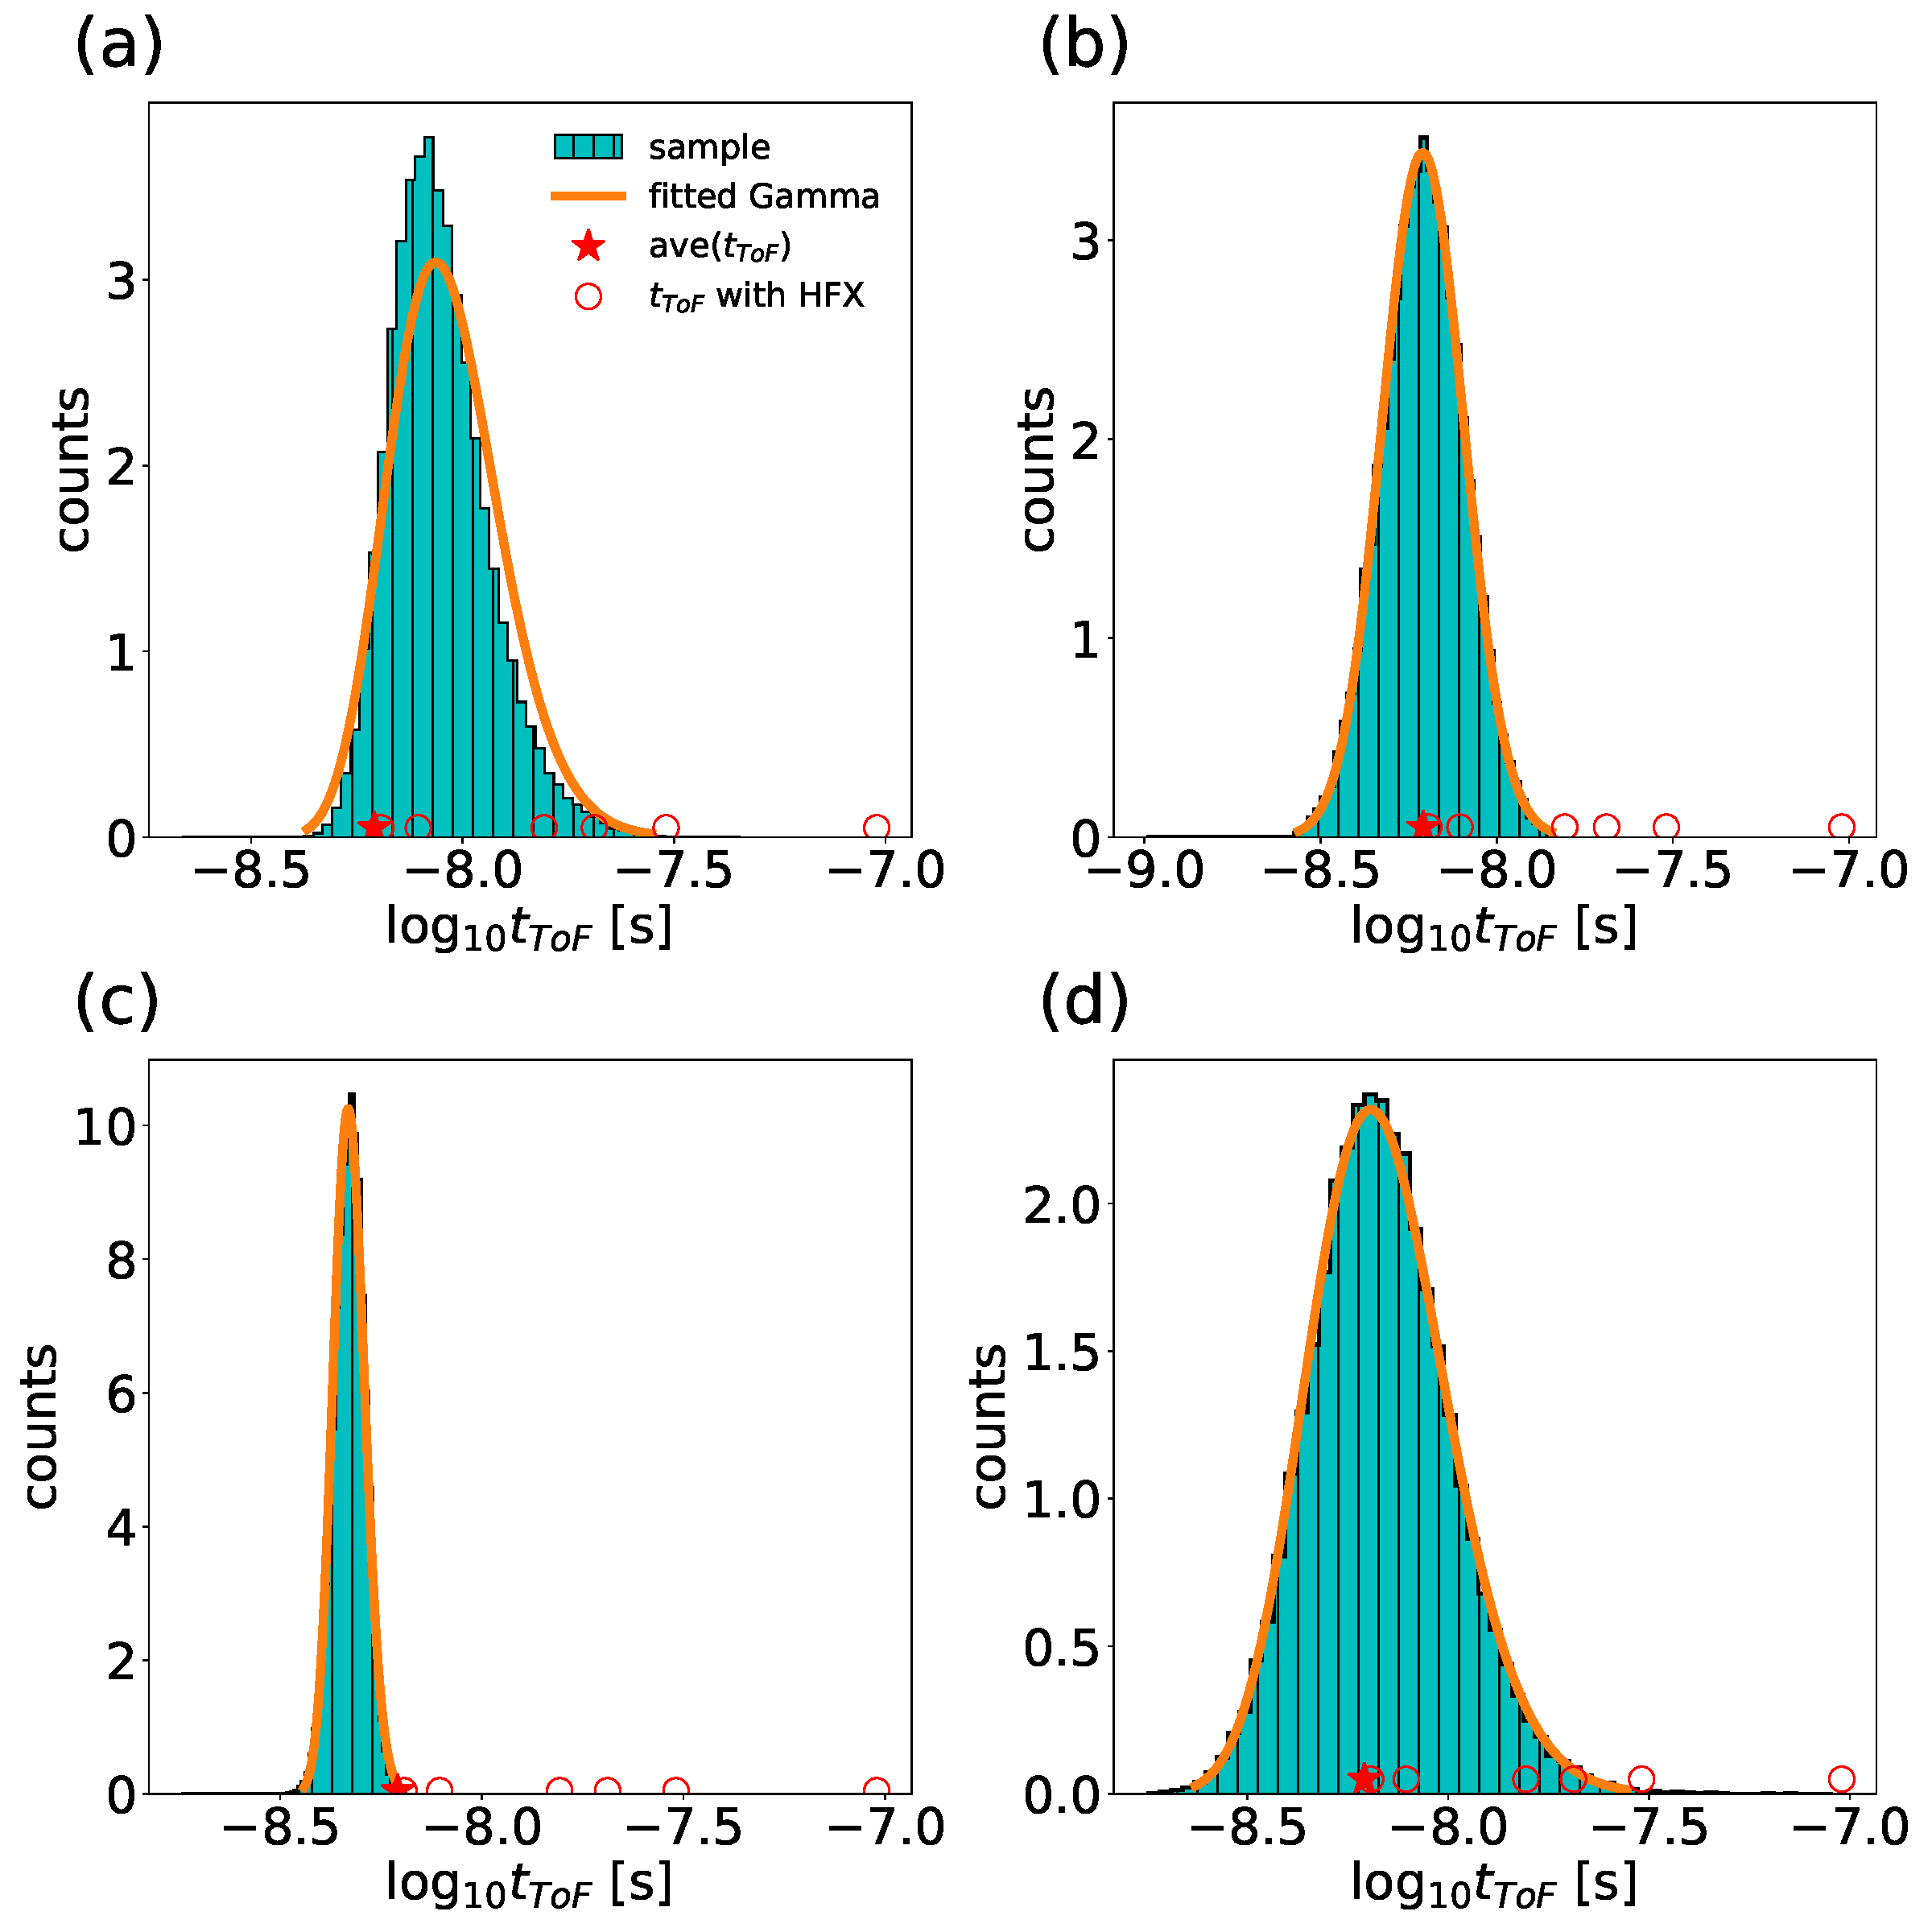
\includegraphics[width=0.75\textwidth]{figs/MADN_HFX/fig_mle_MADN_withE.pdf}
    \caption{Distribution of ToFs in the multiscale modeled MADN system using PBE0 functional and varying HFX. 
    (a) $P(\log_{10}(\tau)|E_i \text{ uncertain})$, 
    (b) $P(\log_{10}(\tau)|\lambda \text{ uncertain})$, 
    (c) $P(\log_{10}(\tau)|J_{ij} \text{ uncertain})$, 
    (d) $P(\log_{10}(\tau)|E_i, \lambda, J_{ij} \text{ uncertain})$. The red star indicates the ToF calculated using the average $\bar{E_i}, \bar{J}_{ij}, \bar{\lambda}$, and the red circles indicate the ToF obtained using different HFX.}
    \label{fig:mle_MADN_withE}
\end{figure}
%

When the energy disorder in MADN system is not considered, that is, all the MADN molecule energy are set to be equal giving $\Delta E=0$, the distribution of ToF is shown in Fig.\ref{fig:mle_MADN_noE}
%
\begin{figure}[H]
    \centering
    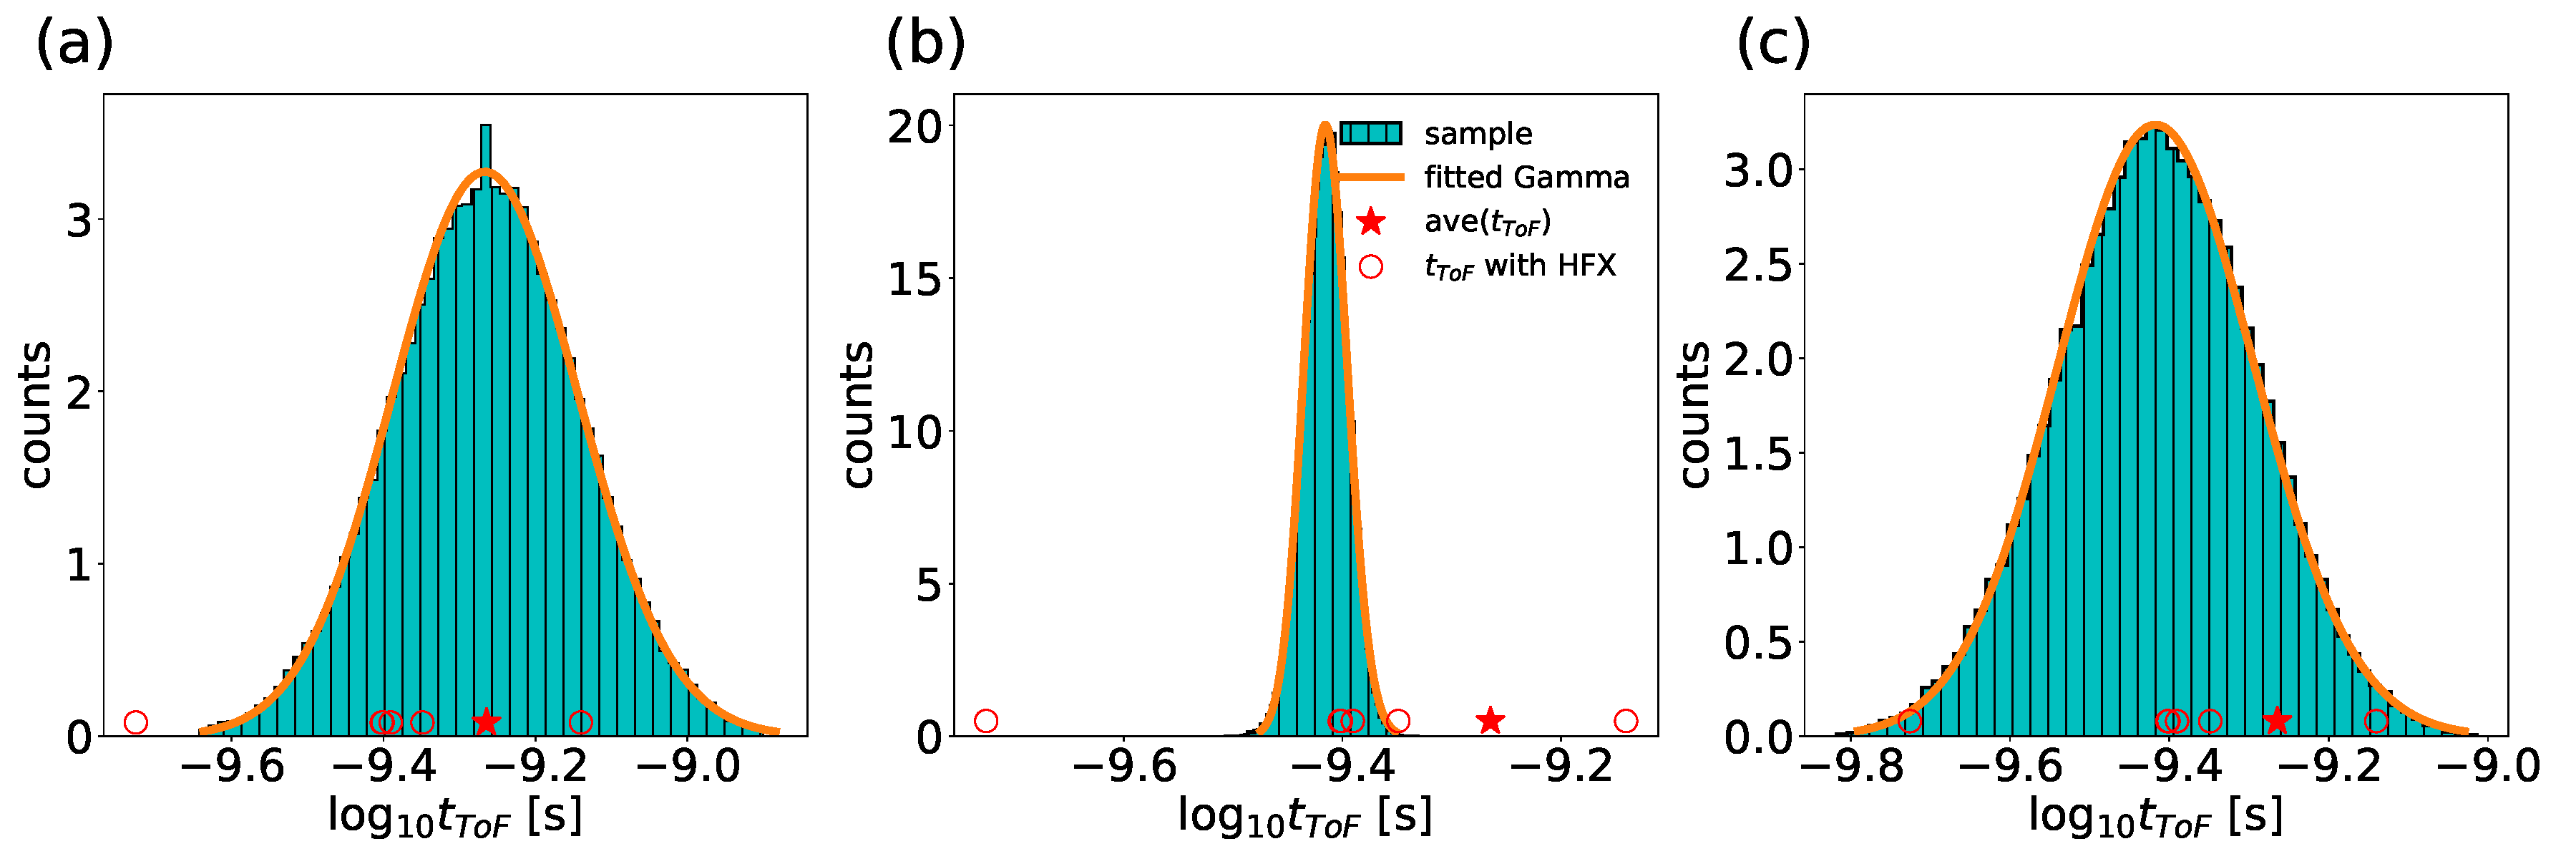
\includegraphics[width=0.99\textwidth]{figs/MADN_HFX/fig_mle_MADN_noE.pdf}
    \caption{Distribution of ToFs in the multiscale modeled MADN system using PBE0 functional and varying HFX. Energy disorder is not consider. 
    (a) $P(\log_{10}(\tau)|\lambda \text{ uncertain})$, 
    (b) $P(\log_{10}(\tau)|J_{ij} \text{ uncertain})$, 
    (c) $P(\log_{10}(\tau)|E_i, \lambda, J_{ij} \text{ uncertain})$. The red star indicates the ToF calculated using the average $\bar{E_i}, \bar{J}_{ij}, \bar{\lambda}$, and the red circles indicate the ToF obtained using different HFX.}
    \label{fig:mle_MADN_noE}
\end{figure}
%


Measuring the sensitivity of each electronic parameter to ToF is to measure each electronic parameter's contribution to the variance of ToF. 
That is, if ToF is most sensitive to one parameter, the variance in this particular parameter will contribute most to the ToF variance. 

One way of decomposing the variance of the model output into fractions attributed to input parameters is the variance-based sensitivity analysis. The local sensitive analysis is to use the partial derivative $\frac{\partial \tau}{\partial x_i}$. While the global sensitivity analysis can use Sobol's indices. Specifically, to measure the parameter $x_i$'s contribution to $\tau$, including all variance caused by its interaction with other parameters $\{x_k, k \neq i \}$, the total effect Sobol's index is calculated as 
\begin{equation}
    S_{Ti} = \frac{ \mathbb{E}_{x_{\sim i}}[ \text{Var}_{x_i}(\tau|x_{\sim i}) ] }{ \text{Var}(\tau) }
    \label{eq:STi}
\end{equation}



\section{Distribution of Steady State Velocity}
The distribution of steady state velocity of MADN is shown as Fig.\ref{fig:mle_MADN_withE_SS} and \ref{fig:mle_MADN_noE_SS}. 
Those distribution shows that the variation in $v_\text{SS}$ distribution is greater than ToF distribution. 

\begin{figure}[H]
    \centering
    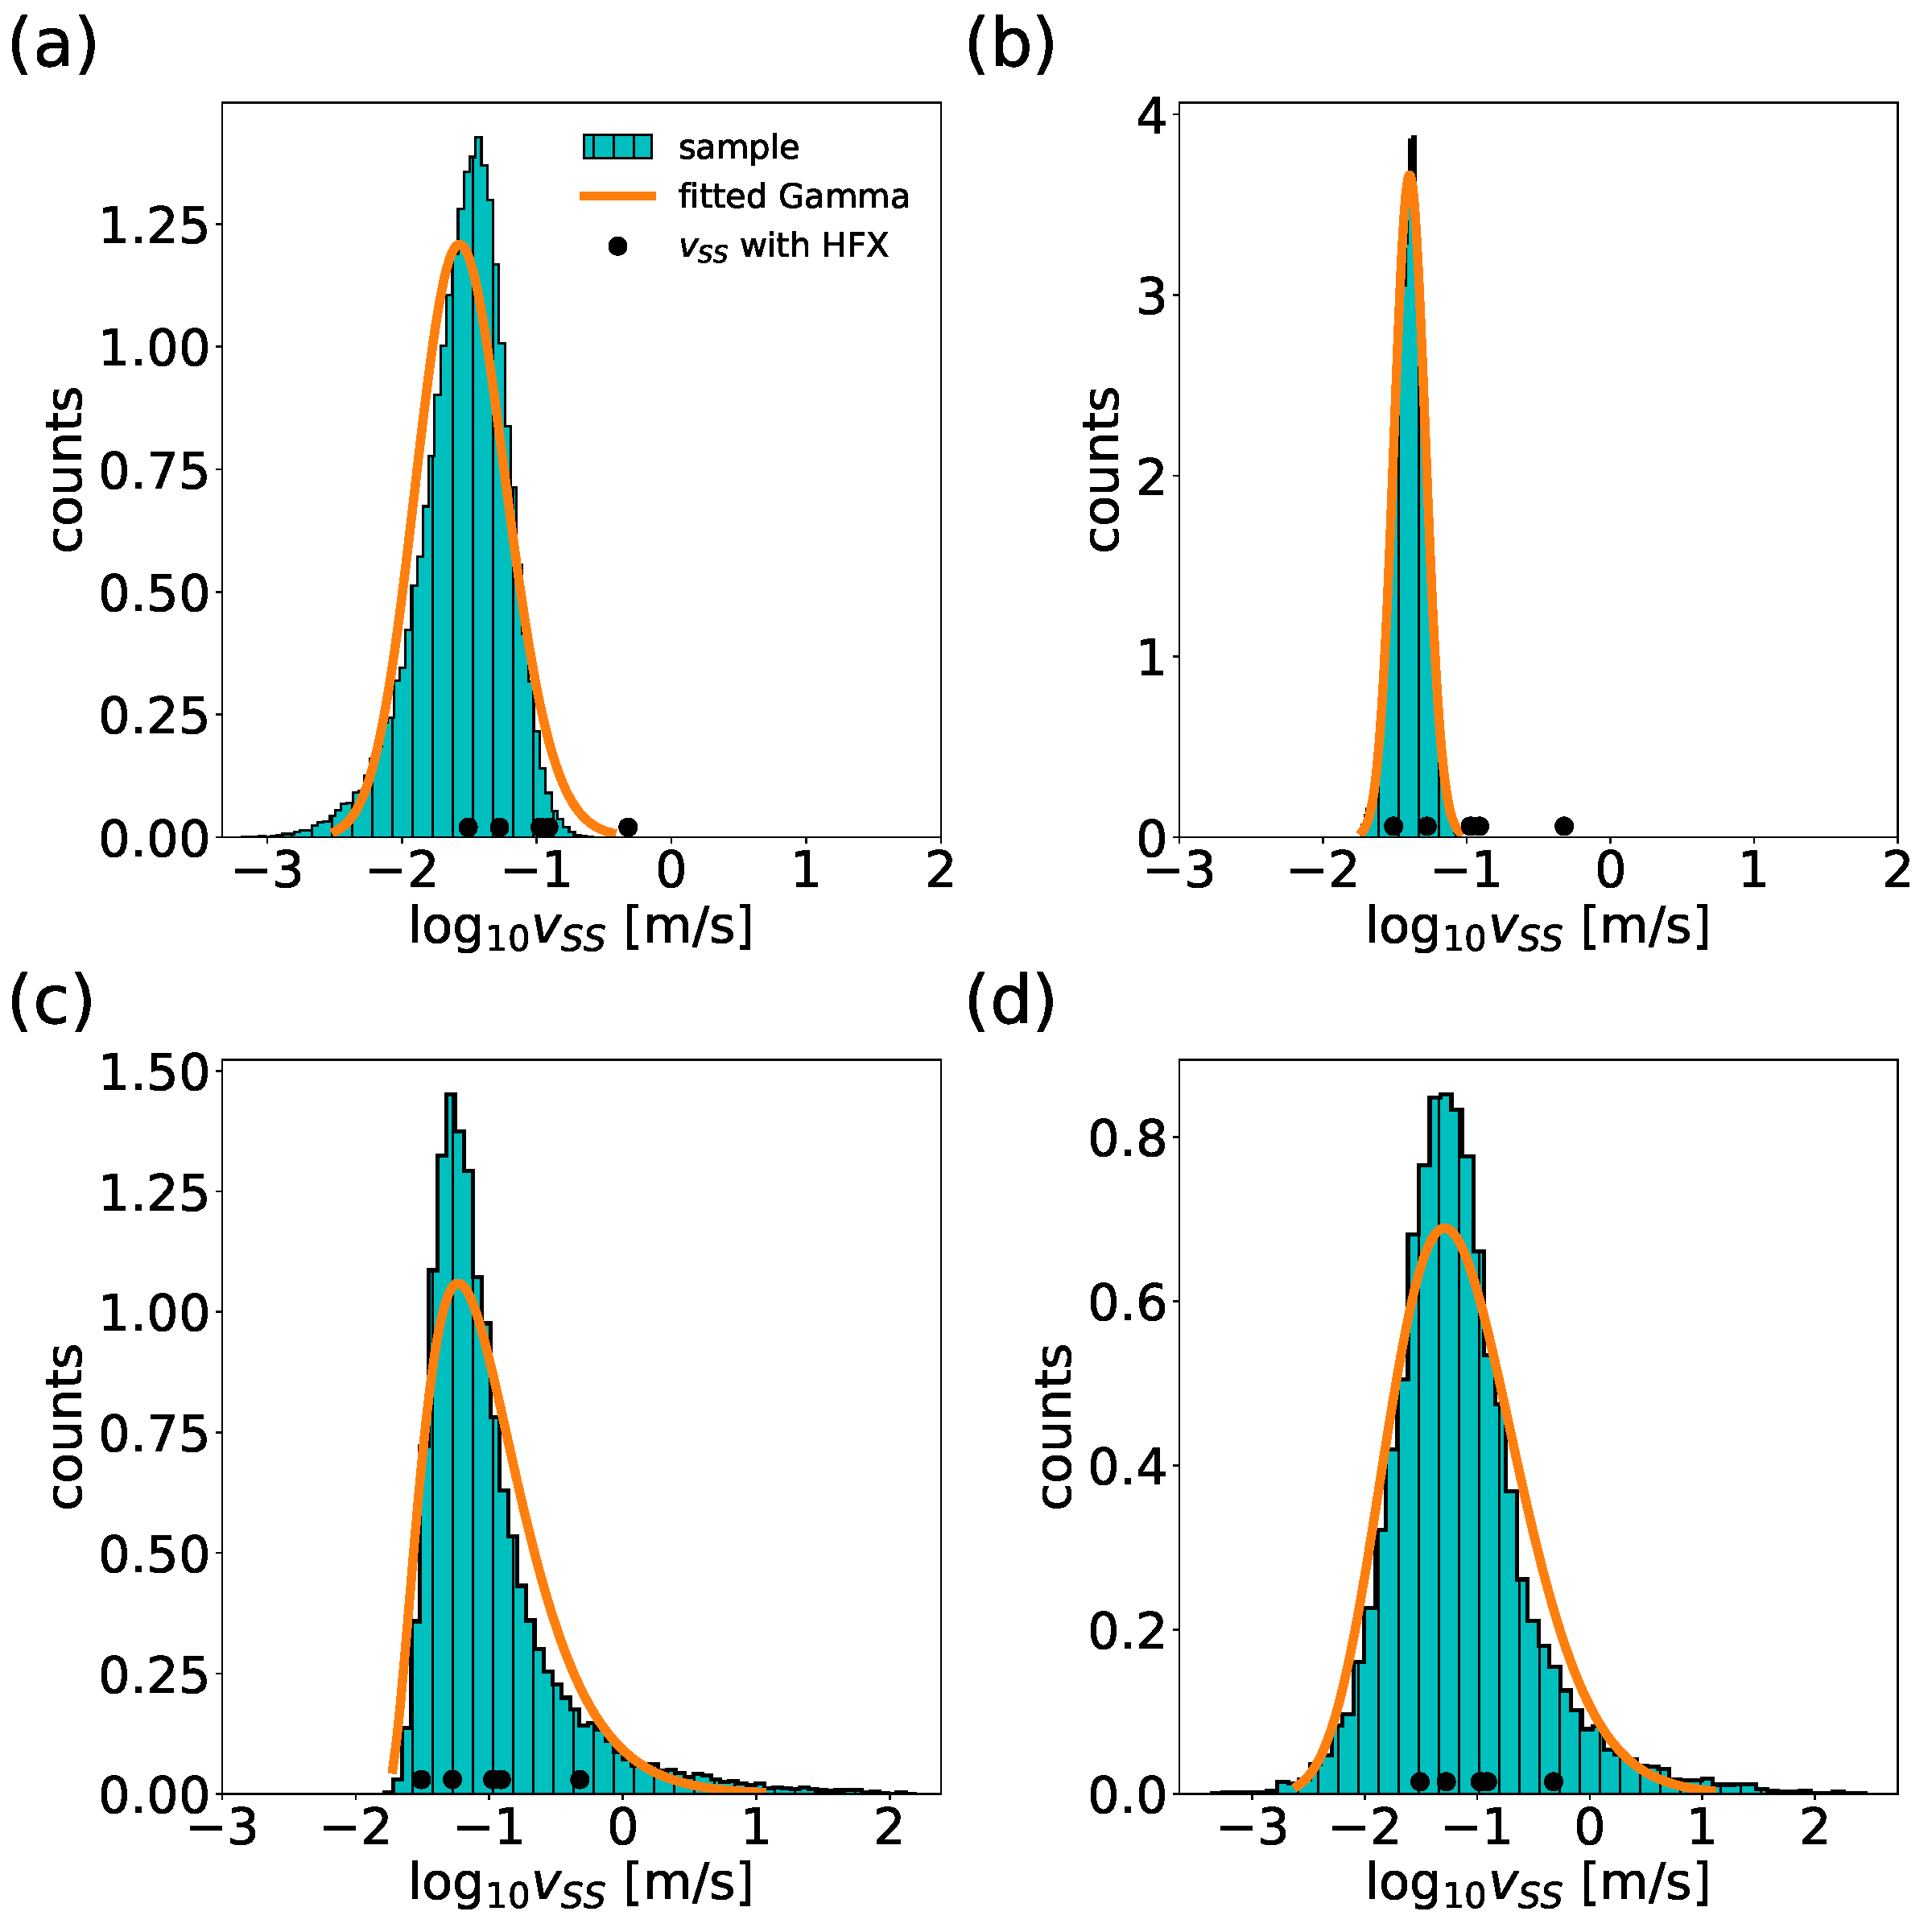
\includegraphics[width=0.8\textwidth]{figs/MADN_HFX/fig_mle_MADN_withE_SS.pdf}
    \caption{Distribution of steady state velocity $v_\text{SS}$ in the multiscale modeled MADN system using PBE0 functional when (a) the molecule site energy $E$ are sampled from a normal distribution $E \sim N(E_\text{ave},E^2_\text{std})$, (b) the reorganization energy $\lambda$ are sampled from a normal distribution $\lambda \sim N(\lambda_\text{ave},\lambda^2_\text{std})$, (c) the quantity $\log_{10}(J^2)$ are sampled from a normal distribution $\log_{10}(J^2) \sim N(\mathbb{E}[\log_{10}(J^2)], \textbf{Var}[\log_{10}(J^2)] )$. (d) Both $E$, $\lambda$ and $\log_{10}(J^2)$ are sampled from the normal distribution. }
    \label{fig:mle_MADN_withE_SS}
\end{figure}

\begin{figure}[H]
    \centering
    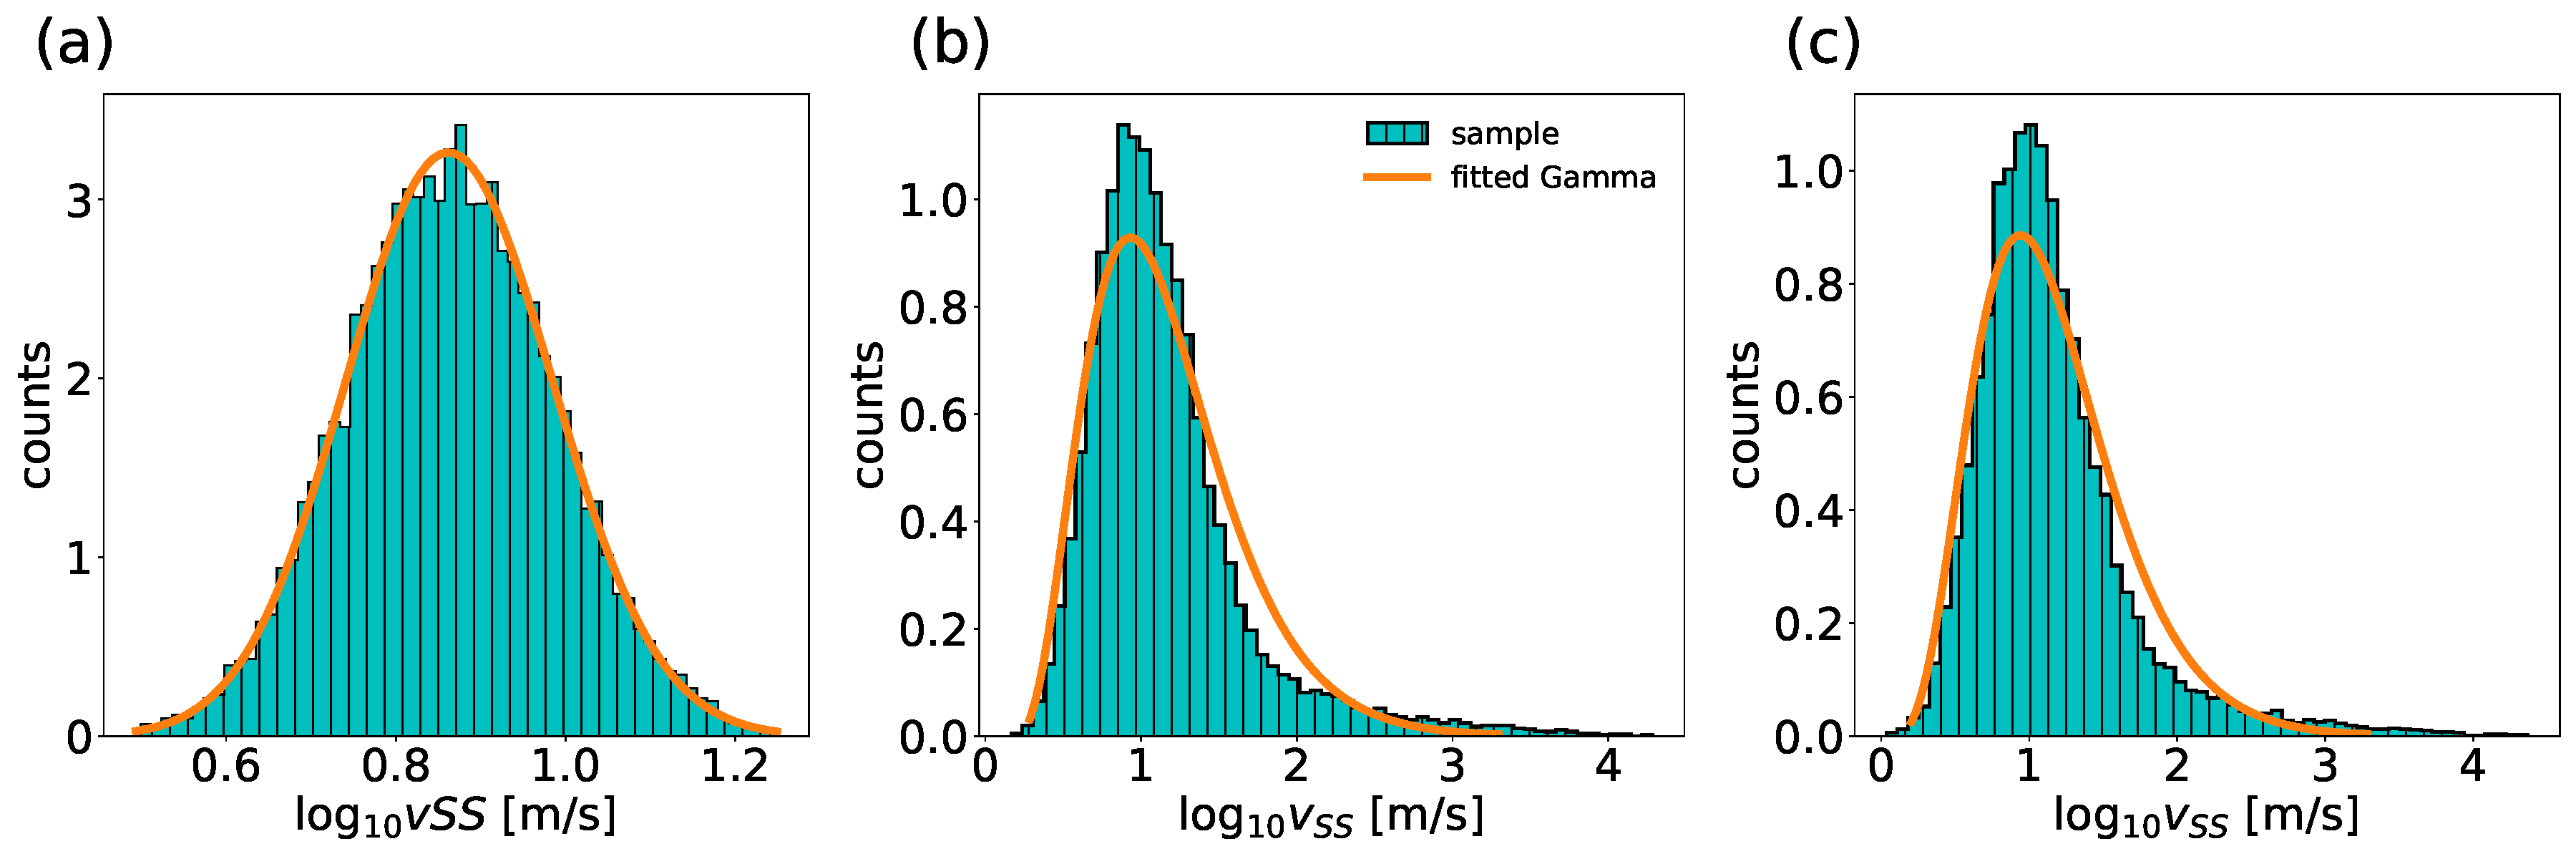
\includegraphics[width=0.99\textwidth]{figs/MADN_HFX/fig_mle_MADN_noE_SS.pdf}
    \caption{Distribution of steady state velocity $v_\text{SS}$ in the multiscale modeled MADN system using PBE0 functional. All molecule energies are set to be zero.  
    The plots are for the situation: (a) The reorganization energy $\lambda$ are sampled from a normal distribution $\lambda \sim N(\lambda_\text{ave},\lambda^2_\text{std})$. (b) the quantity $\log_{10}(J^2)$ are sampled from a normal distribution $\log_{10}(J^2) \sim N(\mathbb{E}[\log_{10}(J^2)], \textbf{Var}[\log_{10}(J^2)] )$. (c) Both $\lambda$ and $\log_{10}(J^2)$ are sampled from the normal distribution. }
    \label{fig:mle_MADN_noE_SS}
\end{figure}
 
%%%%%%%%%%%%%%%%%%%%%%%%%%%%%%%%%%%%%%%%%%%%%%%%%%%%%%%%%%%%%%%%%%%%%%%%%%%%%
\section{Comparison of Diffusive Charge Velocity Between BCP and MADN}
In this section we compare the diffusive charge velocity between BCP and MADN. 
The following tables show the diffusive charge velocity for BCP and MADN with HFX=0.05, 0.15, 0.25. The situations of using energy disorder and without energy disorder are considered.
For the ToF setting, we investigate the situations where the charge transport direction is along the X-axis, Y-axis and Z-axis, as shown in Table \ref{tab:compare_Lx}, \ref{tab:compare_Ly}, and \ref{tab:compare_Lz}. 

The diffusive velocity calculated using steady state setting is $v_\text{SS}$, and the comparison is shown in Table \ref{tab:compare_SS}.
\begin{table}[H]
\centering
\begin{tabular}{c c c c c c c}
    \toprule
     &
        \multicolumn{3}{c}{ with energy $E$} &
        \multicolumn{3}{c}{all $E=0$}  \\
    HFX & MADN & BCP & ratio & MADN & BCP & ratio  \\
    \cmidrule(r){1-7}
    0.05 & $7.87 \times 10^{-9}$ & 0.32 & NA & $4.07 \times 10^{-10}$ & $3.00 \times 10^{-10}$ & NA \\
    0.15 & $3.03 \times 10^{-8}$ & 0.38 & NA & $3.96 \times 10^{-10}$ & $4.67 \times 10^{-10}$ & NA \\
    0.25 & $9.54 \times 10^{-8}$ & 0.026 & NA & $7.24 \times 10^{-10}$ & $7.63 \times 10^{-10}$ & NA \\
    \bottomrule
    \end{tabular}
    \caption{Diffusive $\tau_X$ comparison between multiscale modeled BCP and MADN molecular system with PBE0 functional. The ratio does not apply because the BCP and MADN has different length $L_x$.}
    \label{tab:compare}
\end{table}

\begin{table}[H]
\centering
\begin{tabular}{c c c c c c c}
    \toprule
        &
        \multicolumn{3}{c}{ with energy $E$} &
        \multicolumn{3}{c}{all $E=0$}  \\
    HFX & MADN & BCP & ratio & MADN & BCP & ratio  \\
    \cmidrule(r){1-7}
    0.05 & 1.0 & $2.2 \times 10^{-8}$ & $4.5 \times 10^{7}$ & 19 & 24 & 0.80 \\
    0.15 & 0.31 & $1.8 \times 10^{-8}$ & $1.7 \times 10^{7}$ & 25 & 15 & 1.7 \\
    0.25 & 0.083 & $2.7 \times 10^{-7}$ & $3.1 \times 10^{5}$ & 11 & 9.4 & 1.2 \\
    \bottomrule
    \end{tabular}
    \caption{Diffusive ToF velocity $v_\text{ToF,X}=\frac{L_X}{\tau_X}$ [m/s] comparison between multiscale modeled BCP and MADN molecular system with PBE0 functional. }
    \label{tab:compare_Lx}
\end{table}

\begin{table}[H]
\centering
\begin{tabular}{c c c c c c c}
    \toprule
        &
        \multicolumn{3}{c}{ with energy $E$} &
        \multicolumn{3}{c}{all $E=0$}  \\
    HFX & MADN & BCP & ratio & MADN & BCP & ratio  \\
    \cmidrule(r){1-7}
    0.05 & 0.44 & $5.8 \times 10^{-8}$ & $7.6 \times 10^{6}$ & 17 & 24 & 0.71 \\
    0.15 & 0.057& $1.0 \times 10^{-7}$  & $5.7 \times 10^{5}$ & 17 & 15 & 1.1 \\
    0.25 & 0.041 & $2.8 \times 10^{-7}$ & $1.4 \times 10^{5}$ & 10 & 9.5 & 1.0 \\
    \bottomrule
    \end{tabular}
    \caption{Diffusive ToF velocity $v_\text{ToF,Y}=\frac{L_Y}{\tau_Y}$ [m/s] comparison between multiscale modeled BCP and MADN molecular system with PBE0 functional. }
    \label{tab:compare_Ly}
\end{table}

\begin{table}[H]
\centering
\begin{tabular}{c c c c c c c}
    \toprule
        &
        \multicolumn{3}{c}{ with energy $E$} &
        \multicolumn{3}{c}{all $E=0$}  \\
    HFX & MADN & BCP & ratio & MADN & BCP & ratio  \\
    \cmidrule(r){1-7}
    0.05 & 2.0 & $5.6 \times 10^{-7}$ & $3.4 \times 10^{6}$ & 19 & 24 & 0.80 \\
    0.15 & 2.6 & $1.2 \times 10^{-6}$ & $2.2 \times 10^{6}$ & 19 & 15 & 1.3 \\
    0.25 & 1.0 & $5.4 \times 10^{-6}$ & $1.0 \times 10^{6}$ & 10 & 9.4 & 1.1 \\
    \bottomrule
    \end{tabular}
    \caption{Diffusive ToF velocity $v_\text{ToF,Z}=\frac{L_Z}{\tau_Z}$ [m/s] comparison between multiscale modeled BCP and MADN molecular system with PBE0 functional. }
    \label{tab:compare_Lz}
\end{table}

\begin{table}[htbp]
\centering
\begin{tabular}{c c c c c c c}
    \toprule
        &
        \multicolumn{3}{c}{ with energy $E$} &
        \multicolumn{3}{c}{all $E=0$}  \\
    HFX & MADN & BCP & ratio & MADN & BCP & ratio  \\
    \cmidrule(r){1-7}
    0.05 & 0.10 & $1.5 \times 10^{-7}$ & $6.7 \times 10^{5}$ & 3.8 & 2.4 & 1.6 \\
    0.15 & 0.031 & $1.5 \times 10^{-8}$ & $2.1 \times 10^{6}$ & 13 & 0.58 & 22 \\
    0.25 & 0.0043 & $3.6 \times 10^{-7}$ & $1.2 \times 10^{4}$ & 4.0 & 1.07 & 3.7 \\
    \bottomrule
    \end{tabular}
    \caption{Steady state diffusive velocity $v_\text{SS}$ [m/s] comparison between multiscale modeled BCP and MADN molecular system with PBE0 functional. }
    \label{tab:compare_SS}
\end{table}

%%%%%%%%%%%%%%%%%%%%%%%%%%%%%%%%%%%%%%%%%%%%%%


\bibliographystyle{unsrt}
\bibliography{references}

\begin{comment}
\textbf{Point 1:} To investigate the effect of different functionals $f^\text{DFT}$ on electronic structures, we compare the energies $E_i$ and couplings $J_{ij}$ for all molecule indices $i,j$. Scatter plots in Figures \ref{fig:scatterE} and \ref{fig:scatterJ} illustrate these comparisons.

\begin{figure}[h]
    \centering
    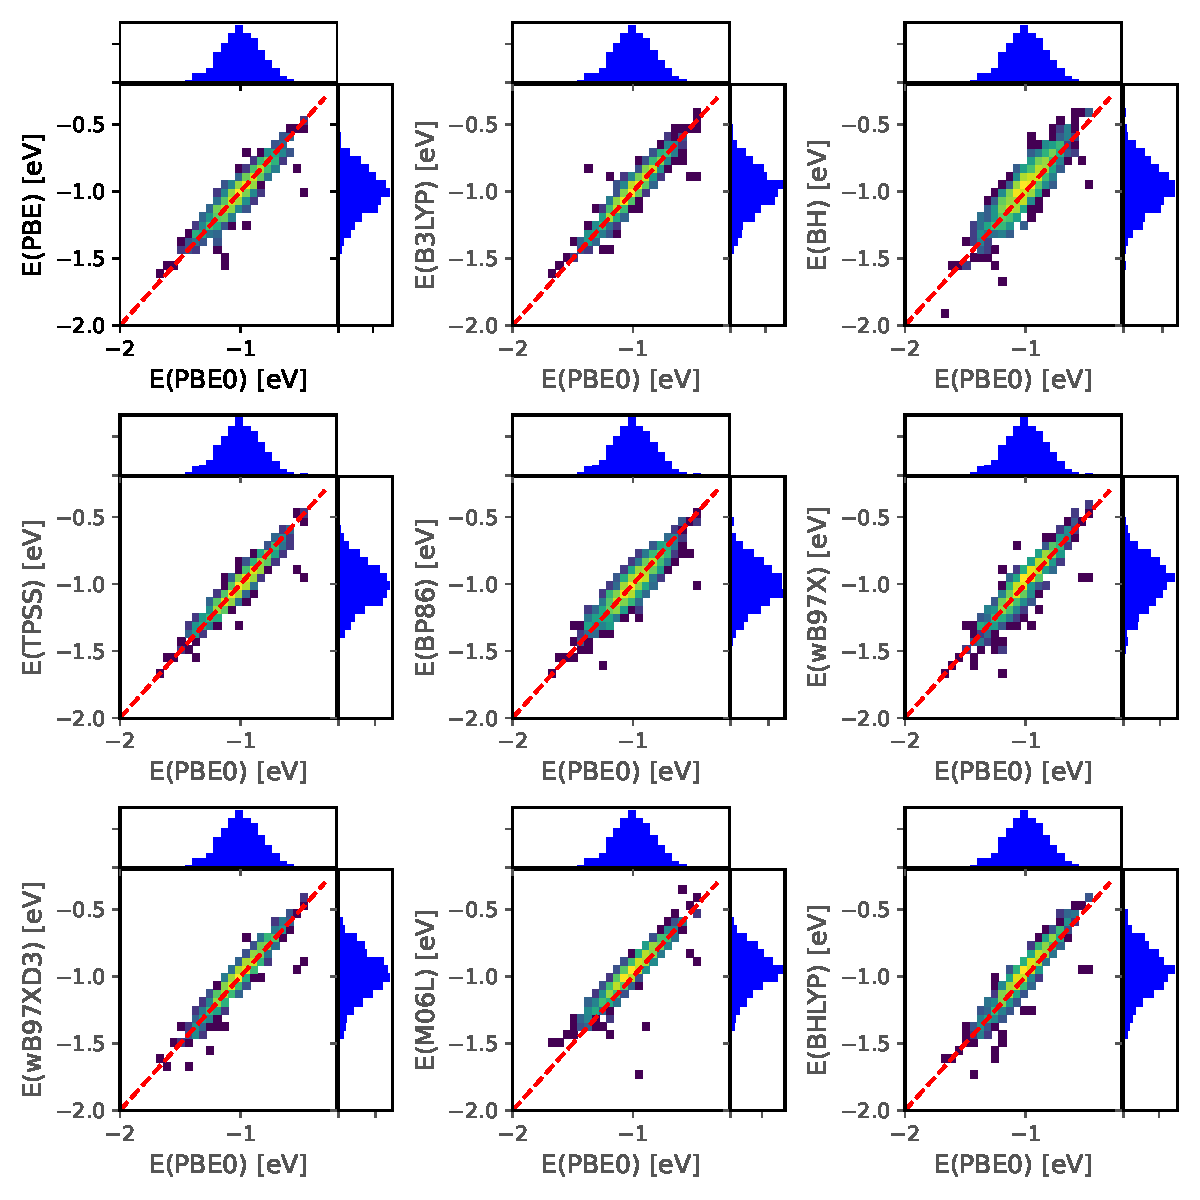
\includegraphics[width=0.95\textwidth]{figs/scatterE_all.pdf}
    \caption{Energy heat maps: $X$-axis shows energies of BCP molecules obtained using PBE0, while the $Y$-axis shows energies from a different functional $f'$.}
    \label{fig:scatterE}
\end{figure}

\begin{figure}[h]
    \centering
    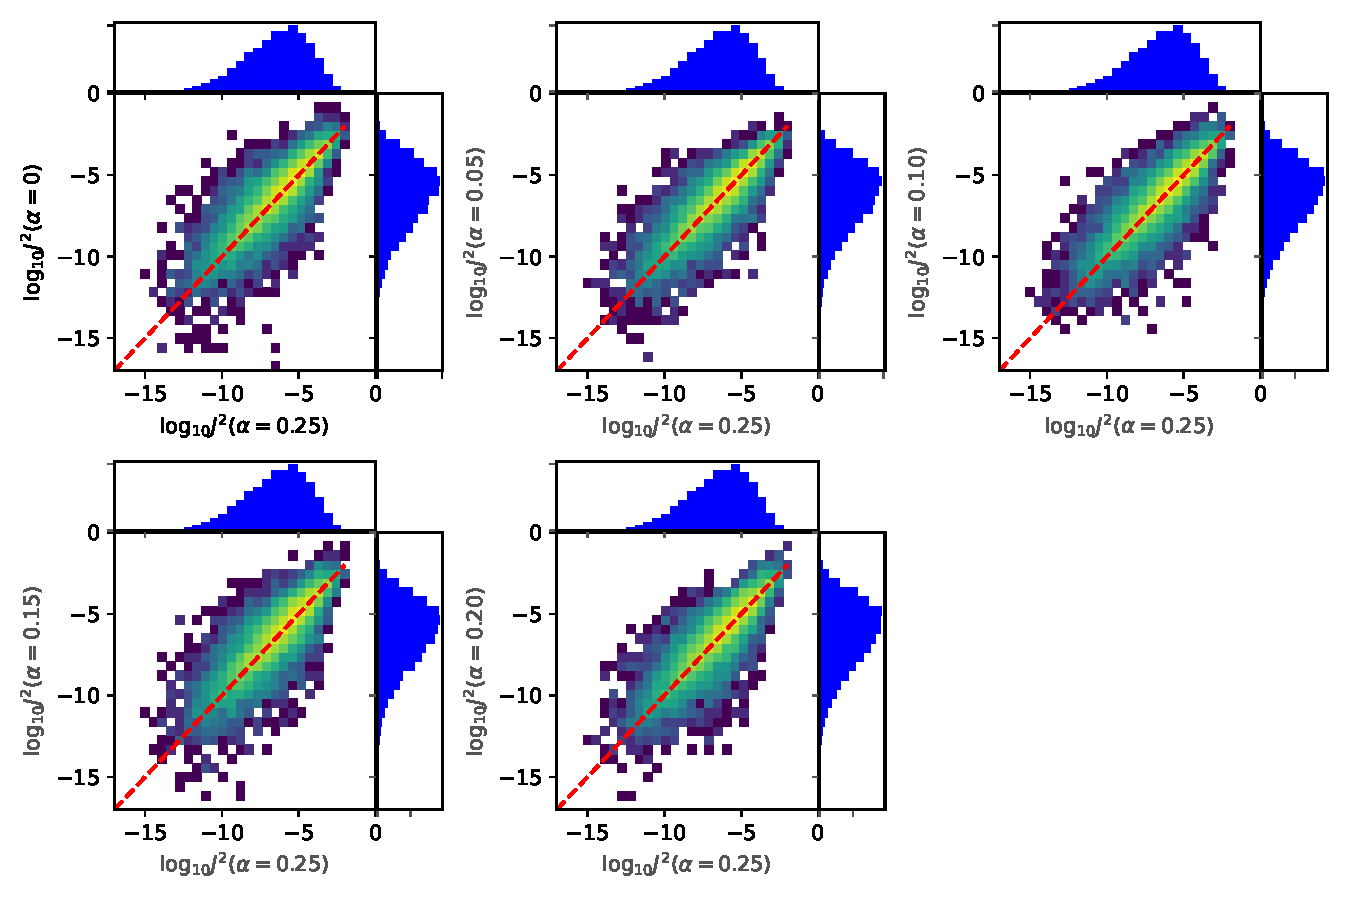
\includegraphics[width=0.95\textwidth]{figs/scatterJ_all.pdf}
    \caption{Scatter heat maps of $\log_{10}(J^2)$: $X$-axis shows $\log_{10}(J^2)$ of BCP molecules obtained using PBE0, while the $Y$-axis shows $\log_{10}(J^2)$ from a different functional $f'$.}
    \label{fig:scatterJ}
\end{figure}

\textbf{Point 2:} Both $E_i$ and $J_{ij}$ are distributions. To quantify the impact of these distributions on $\Delta$ToF, we plot the Wasserstein distance versus $\Delta$ToF. Figure \ref{fig:distance_ToF} shows that different functionals generate similar energy sets, but $\Delta$ToF is not correlated with energy distribution distance.

\begin{figure}[h]
    \centering
    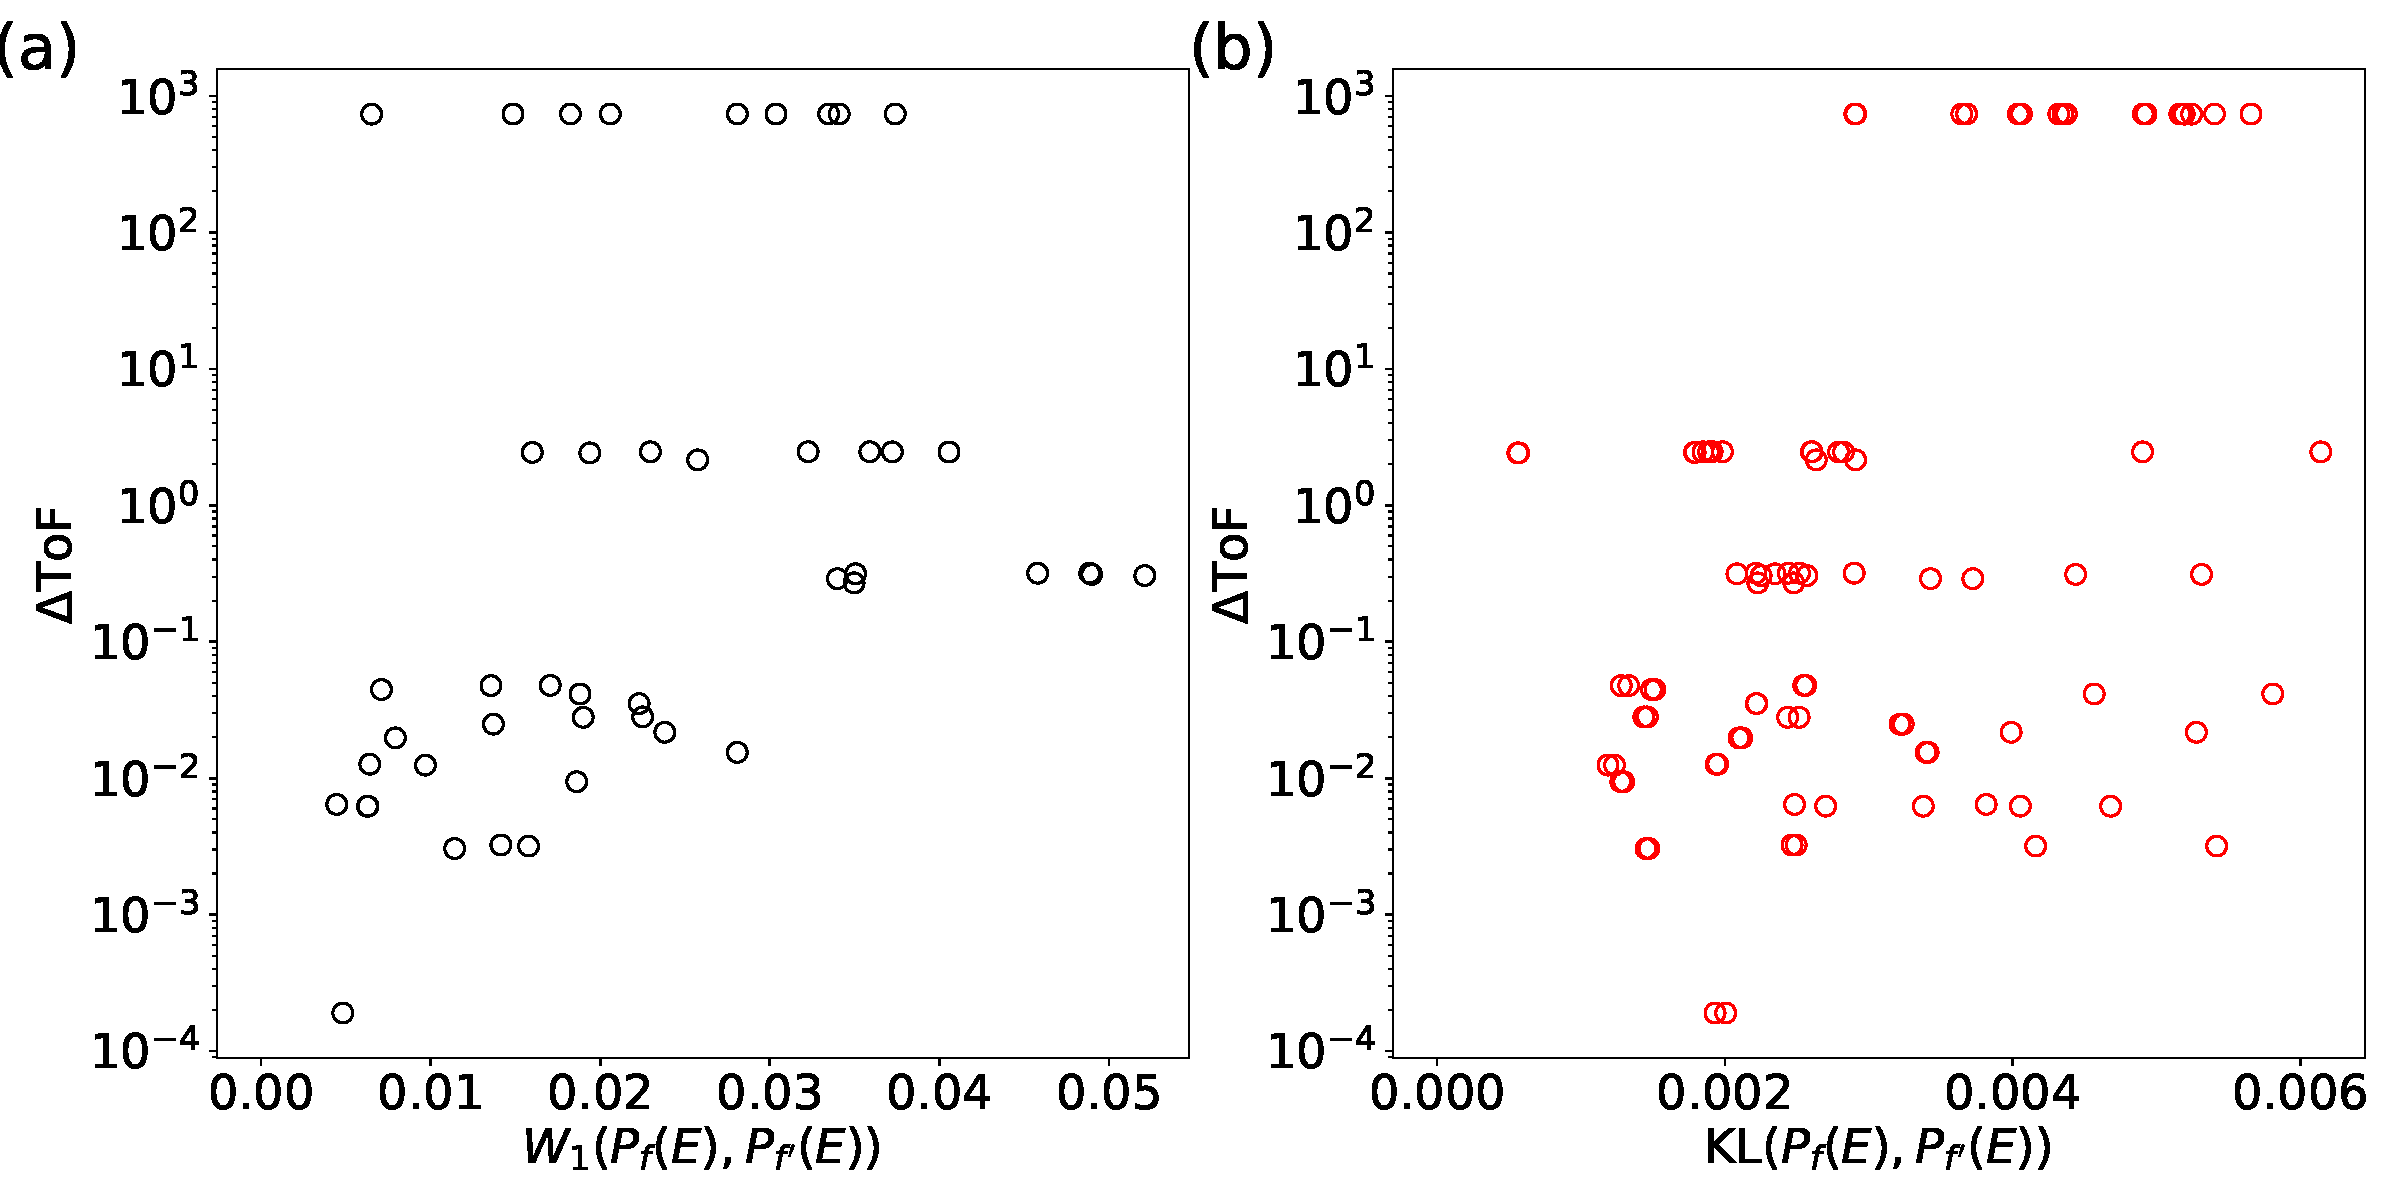
\includegraphics[width=0.9\textwidth]{figs/DeltaToF_W_KL_E.pdf}
    \caption{Left: scatter plot of $W_1(P_f,P_{f'})$ vs. $\Delta$ToF. Right: scatter plot of $KL(P_f(E),P_{f'}(E))$ vs. $\Delta$ToF.}
    \label{fig:distance_ToF}
\end{figure}

\textbf{Point 3:} We then examine other rate-related parameter distributions, calculating the Wasserstein distance and plotting against $\Delta$ToF. Figure \ref{fig:d_WD_tof} reveals that only the rate $P_f(\omega)$ has a large Wasserstein distance when varying $f^\text{DFT}$; other parameters show similar distributions.

\begin{figure}[h]
    \centering
    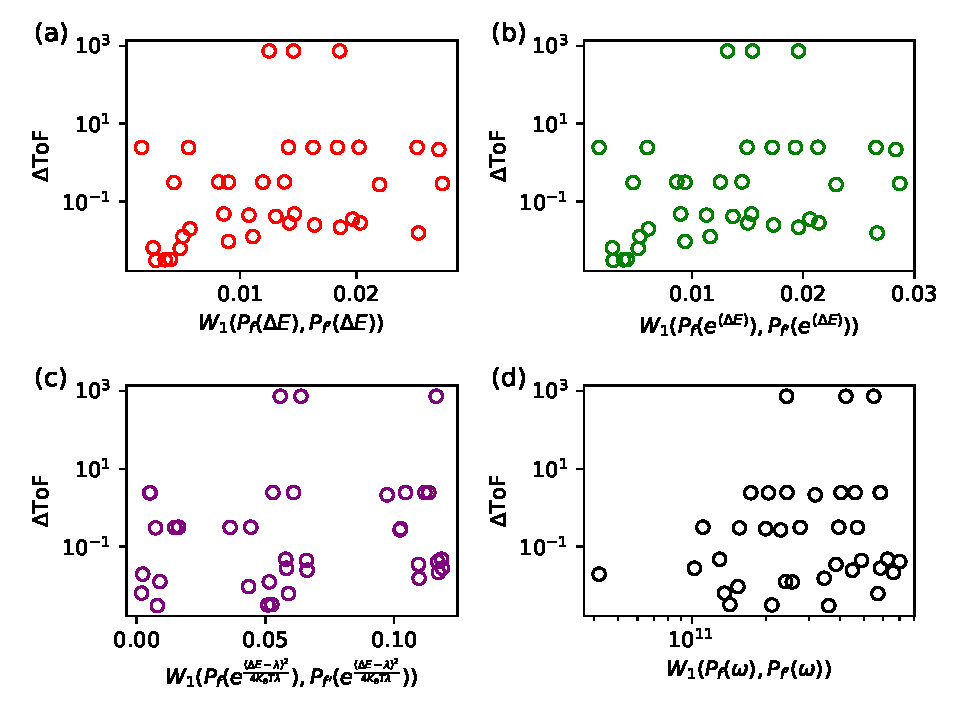
\includegraphics[width=0.7\textwidth]{figs/DeltaToF_W_all.pdf}
    \caption{Scatter plots of (a): $W_1(P_f(\Delta E),P_{f'}(\Delta E))$, (b): $W_1(P_f(\exp(\Delta E)),P_{f'}(\exp(\Delta E)))$, (c): $W_1(P_f(\exp \frac{-(\Delta E - \lambda)^2}{4 k_B T \lambda}),P_{f'}(\exp \frac{-(\Delta E - \lambda)^2}{4 k_B T \lambda}))$, and (d): $W_1 (P_f(\omega), P_{f'}(\omega) )$ vs. $\Delta$ToF.}
    \label{fig:d_WD_tof}
\end{figure}


\textbf{Point4:} Although $f^\text{DFT}$ affects $P_f(\omega)$, but we further notice that $\Delta$ToF is not correlated to its Wasserstein distance. 
So we hypothesize that the connectivity of the graph changed due to different $f^\text{DFT}$. The connectivity of the graph is quantified by the second eigenvector of the graph Laplacian, so we make the figure to investigate the correlation between the $\Delta$ToF and the graph connectivity. 
Figure .\ref{fig:d_eig_tof} shows the ratio of $f^\text{DFT}$ and the second eigenvalue ratio between the graph Laplacian. These two quantities look correlated, and we calculate the Spearman rank coefficient, which is shown in Table.\ref{tab:spearman}.

\begin{table}[h]
    \centering
    \begin{tabular}{c c c}
    \hline
        Data Set & Spearman Rank Coefficient & $p$-value \\ 
        \hline
        $\frac{\lambda_{2,L_W}(f)}{\lambda_{2,L_W}(f')}$ vs $\frac{\text{ToF}(f)}{\text{ToF}(f')}$ & -0.57 & 4.6e-5 \\
        $\frac{\lambda_{2,L_\text{rw}}(f)}{\lambda_{2,L_\text{rw}}(f')}$ vs $\frac{\text{ToF}(f)}{\text{ToF}(f')}$ & -0.38 & 9.4e-3 \\ 
    \hline
    \end{tabular}
    \caption{Spearman rank coefficients for the relationship between $\frac{\lambda_2(f)}{\lambda_2(f')}$ and $\frac{\text{ToF}(f)}{\text{ToF}(f')}$}
    \label{tab:spearman}
\end{table}

\begin{figure}[h]
    \centering
    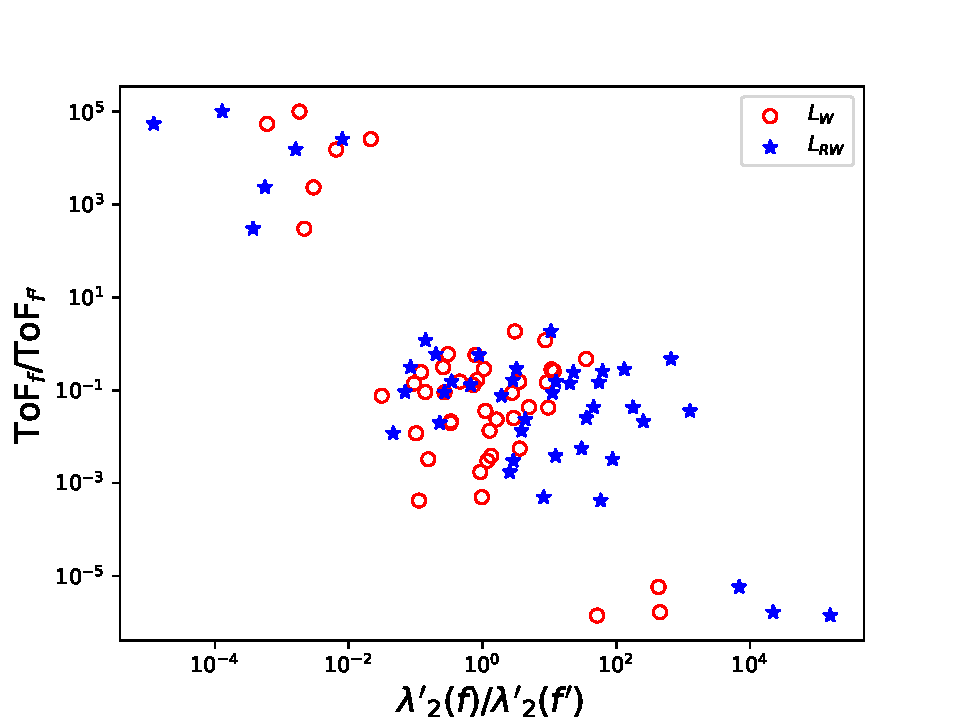
\includegraphics[width=0.6\textwidth]{figs/ratio_tof_2ndEigval.pdf}
    \caption{Scatter plot of $\frac{\lambda_{2}(f)}{\lambda_{2}(f')}$ vs. $\frac{\text{ToF}(f)}{\text{ToF}(f')}$}
    \label{fig:d_eig_tof}
\end{figure}


\textbf{Point5:} The eigenvalue comes in pair with the eigenvector, so we further investigated the corresponding second eigenvector element distributions, as shown in Fig.\ref{fig:2ndVecLW}. 
To our surprise, node 66 has very different second eigenvector entries, so we performed K-means partitioning on those second eigenvector elements.

\textbf{Point6:} After partitioning, we notice that the partition cost function is correlated to $\Delta$ToF.
This correlation shows that the $\Delta$ToF correlated to the connectivity of the graph, althouth the electronic structures and rate-related parameters are similar. 

\begin{figure}
    \centering
    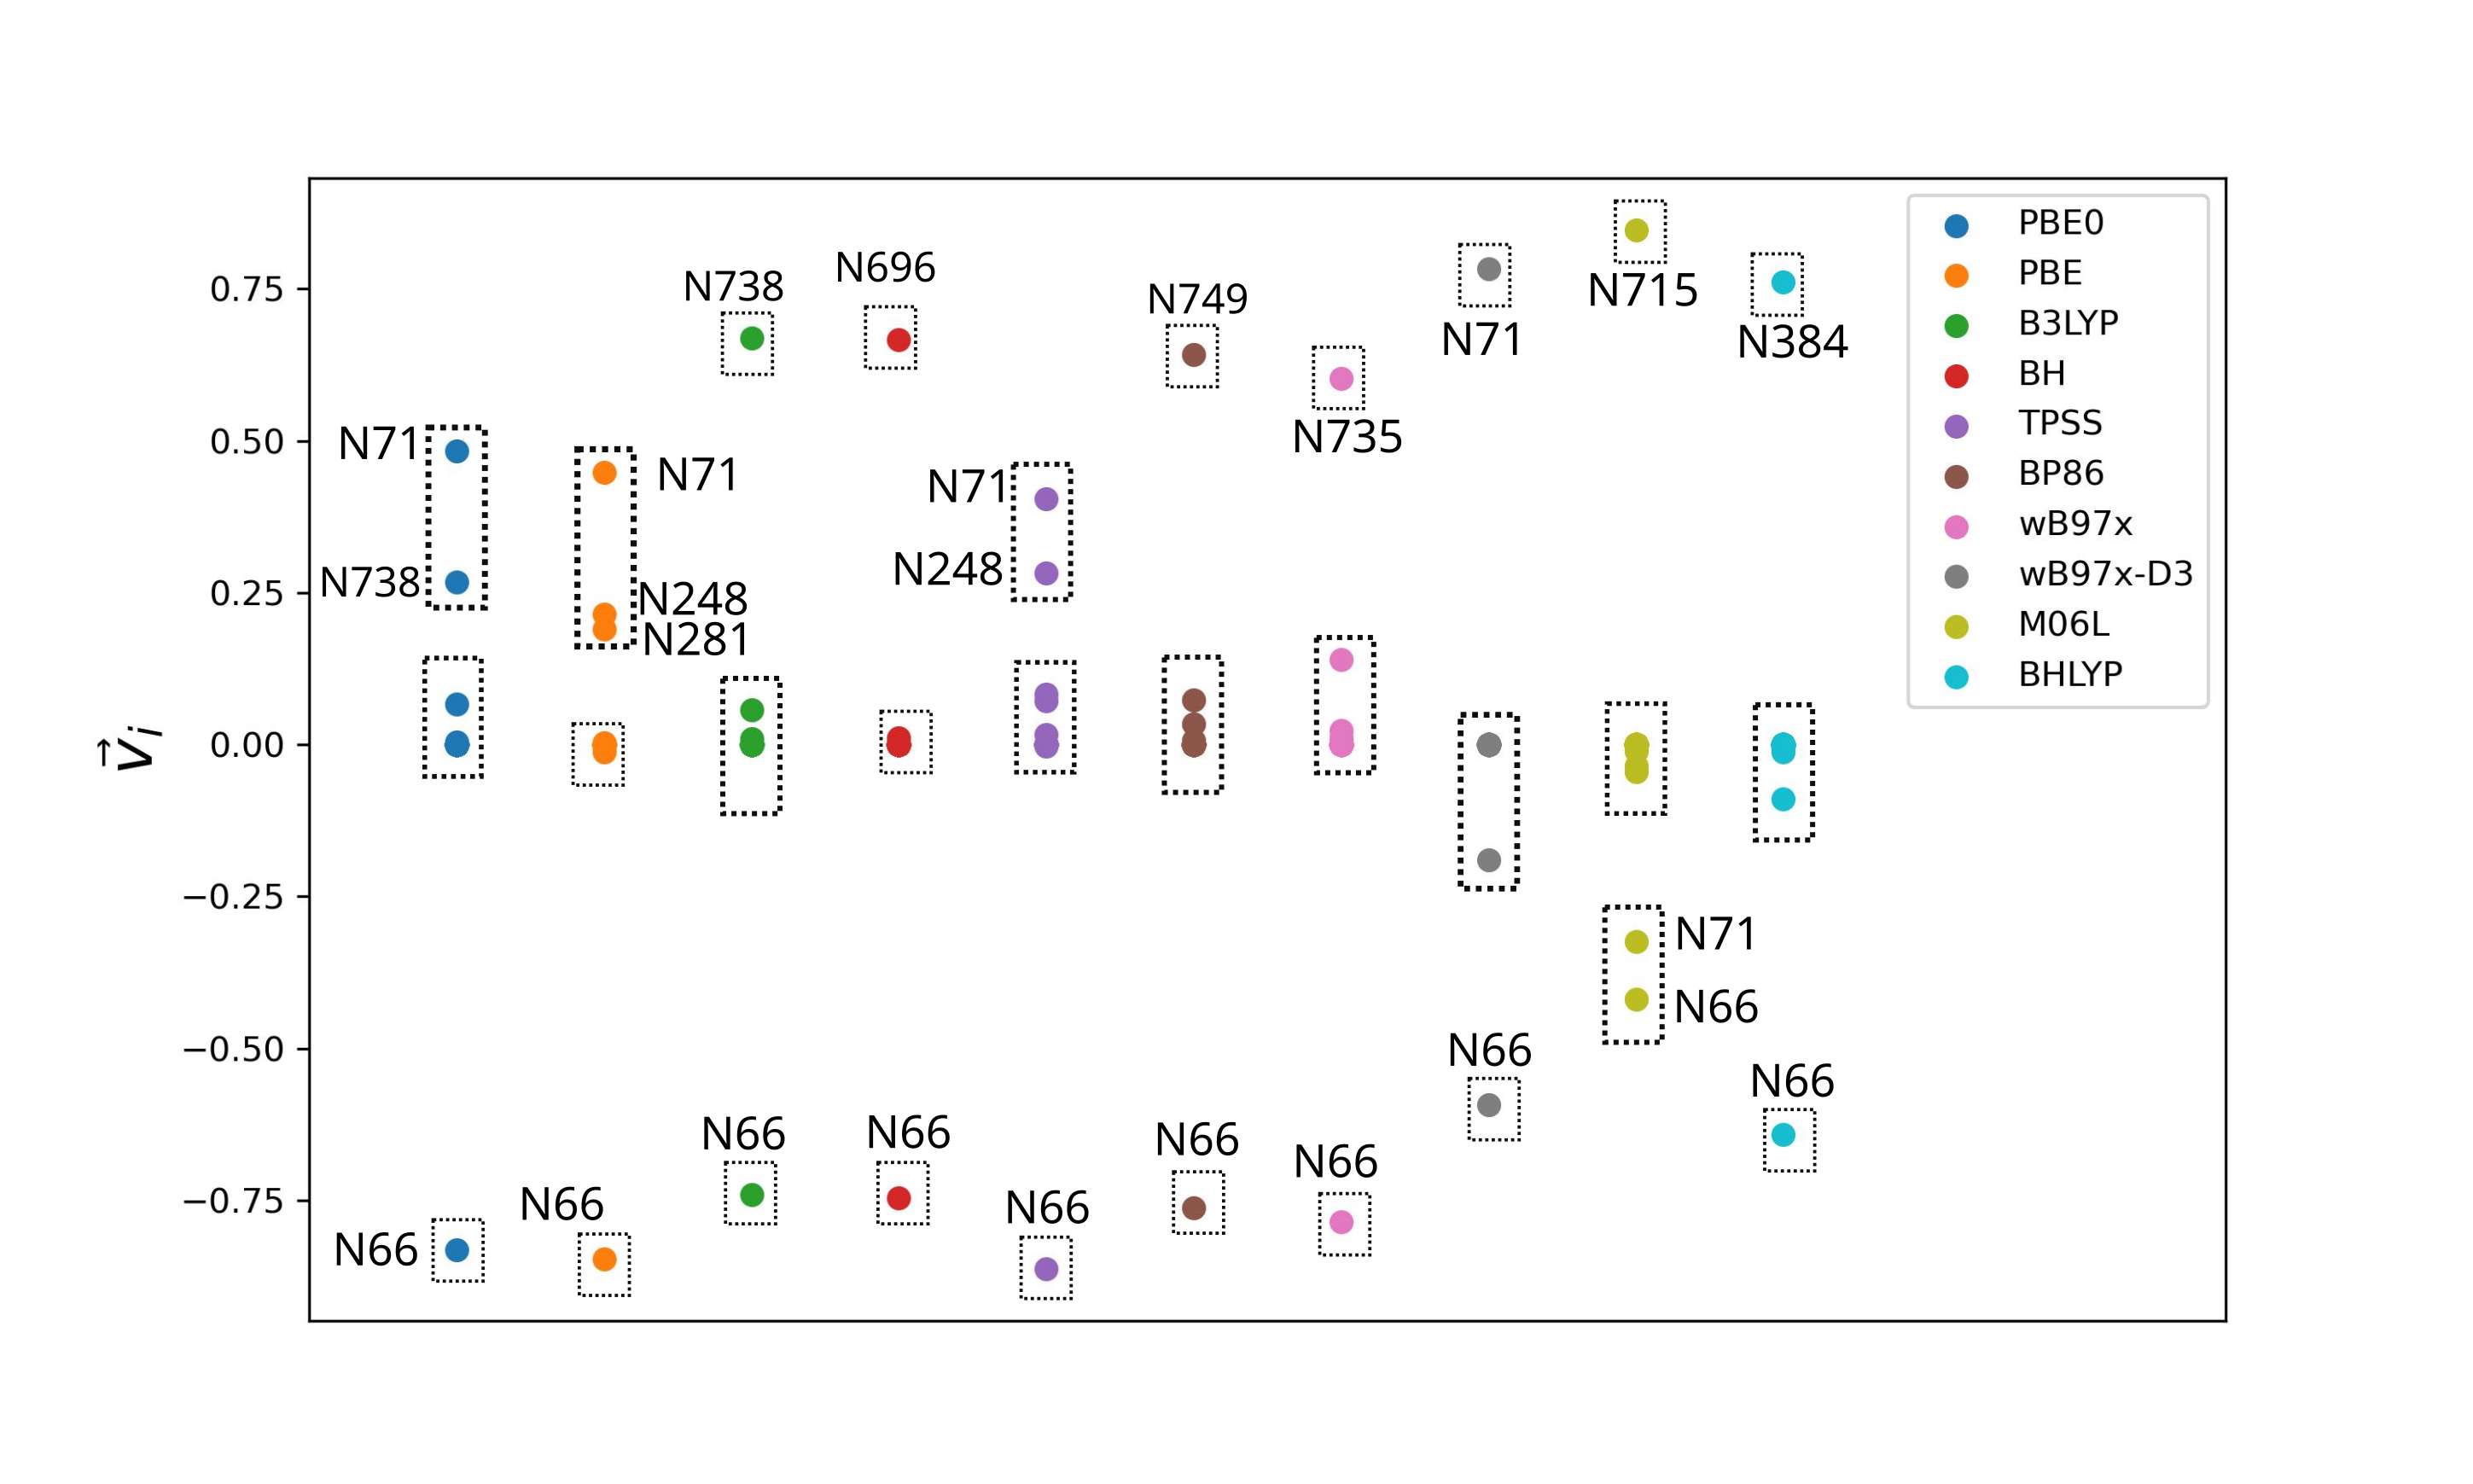
\includegraphics[width=0.8\textwidth]{figs/fig_2ndVecLw.png}
    \caption{Scatter plot of the eigen vector entries $\Vec{v}_i$ of $L_W$ for various $f$ indicated by the legend and point color. 
    The numbers are node index. The dash rectangular indicates the 3-means clusters that are detected as clusters by the Kmeans Lloyd's algorithm. }
    \label{fig:2ndVecLW}
\end{figure}

\begin{figure}
    \centering
    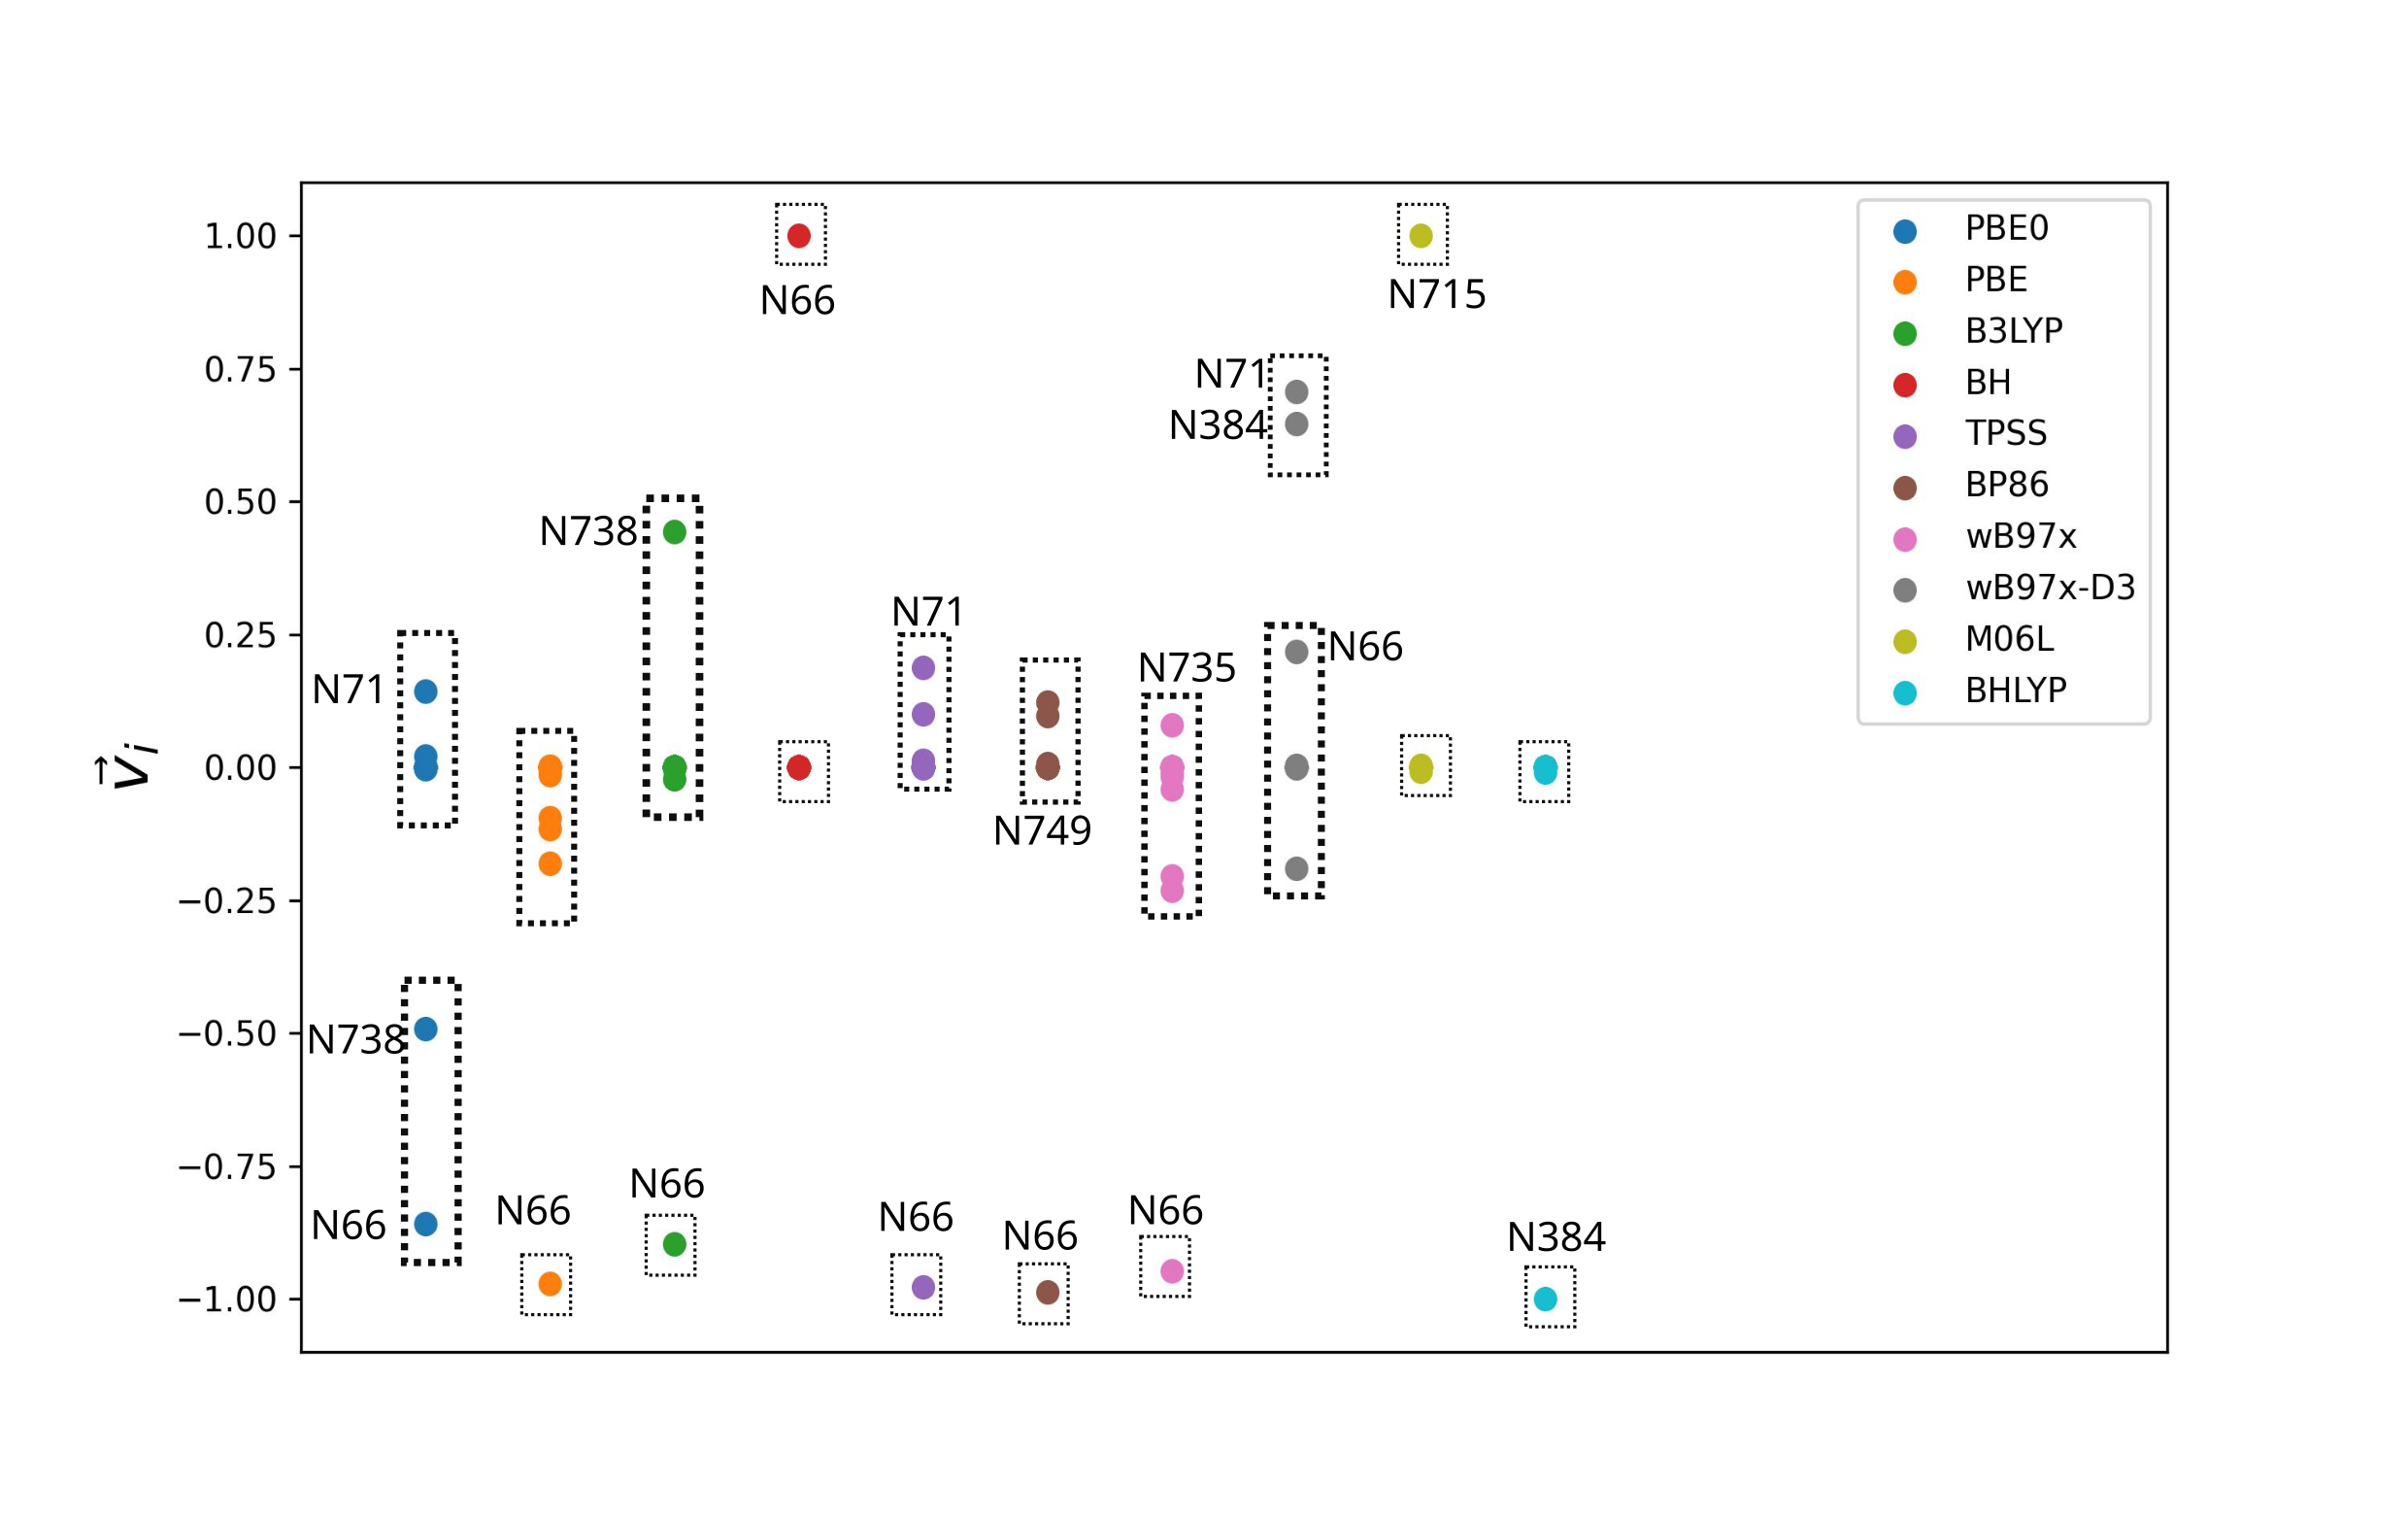
\includegraphics[width=0.8\textwidth]{figs/fig_2ndVecRW.png}
    \caption{Scatter plot of the eigen vector entries $\Vec{v}_i$ of $L_{rw}$ for various $f$ indicated by the legend and point color. 
    The numbers are node index. The dash rectangular indicates the 3-means clusters that are detected as clusters by the Kmeans Lloyd's algorithm.  }
    \label{fig:2ndVecRW}
\end{figure}


Figure \ref{fig:fig_Z_ToF} shows scatter plots of K-means clustering partition cost $Z_{2c}, Z_{3c}$ versus ToF. For the normal Laplacian $L_w$, $Z_{2c}$ is not correlated with the ToF, but $Z_{3c}$ is. For the Random-walk Laplacian, both $Z_{2c}$ and $Z_{3c}$ show a strong correlation with ToF. Thus, the clustering cost function indicates the speed of charge dynamics as measured by ToF.

\begin{figure}
    \centering
    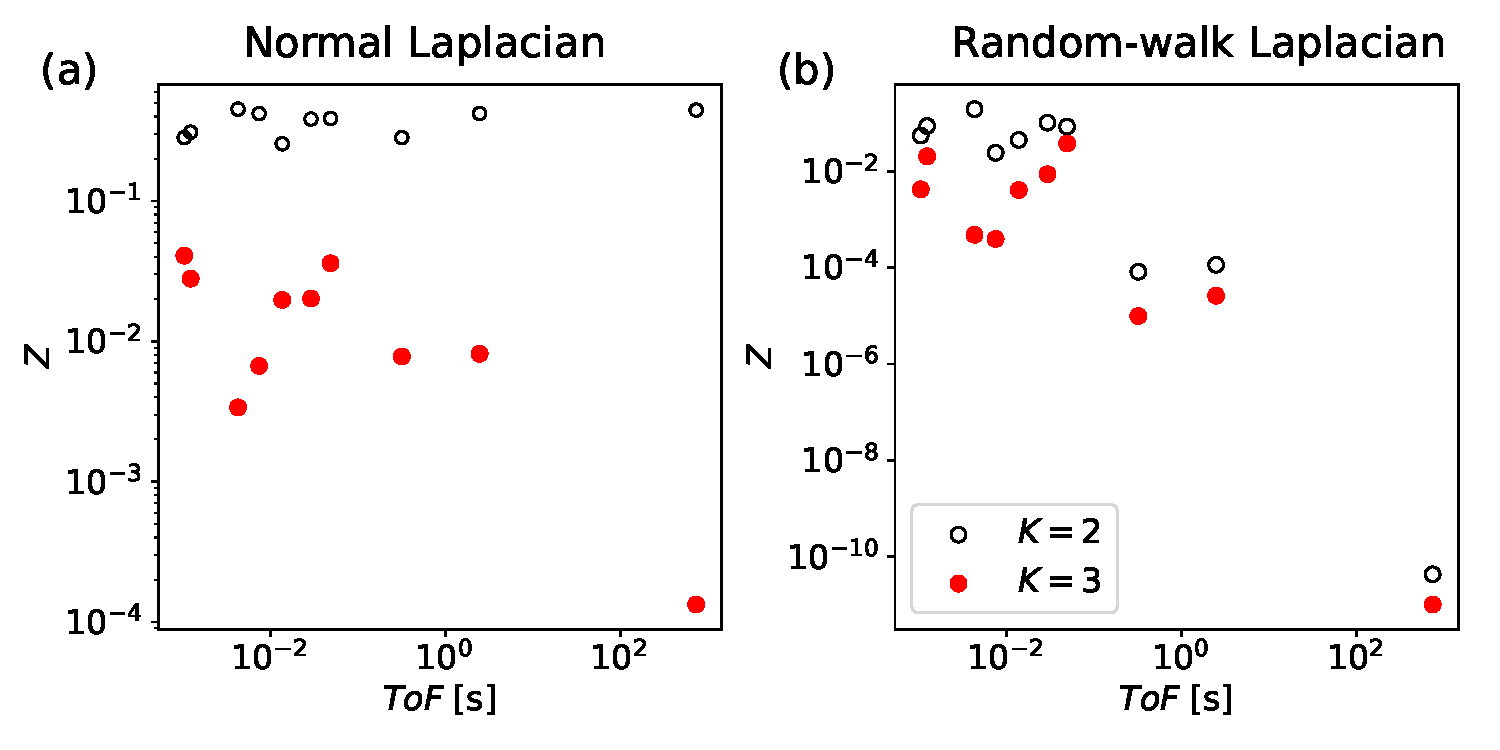
\includegraphics[width=0.9\textwidth]{figs/fig_Z_ToF.pdf}
    \caption{Scatter plot of $Z$ vs $\text{ToF}$. (a): K-means partition of the second eigenvector of $L_W$ for $K=2$ and $K=3$ (b) K-means partition of the second eigenvector of $L_{RW}$ for $K=2$ and $K=3$}
    \label{fig:fig_Z_ToF}
\end{figure} 


\textbf{Point7:} Now that the ToF has a large range, we want to know which ToF to trust.  And for application purposes, a very important message is to know what the range of ToF will give a 90\% confidence level. 

Since we do not really know the exchange-correlation potential, we assume that for each molecule, the uncertainty in its energy $E_i$ is represented by a normal distribution $E_i \in N(\bar{E_i},\sigma(E_i))$. Normal distribution is used because the normal distribution encodes the maximum amount of uncertainty over the real numbers out of all possible probability distributions with the same variance. 
So the normal distribution inserts the least amount of prior knowledge into our model. 
So we experiment: 

\textbf{Point8:} For each molecule energy $E_i$, we use maximum likelihood estimation to obtain the $N(\bar{E_i},\sigma(E_i))$. Then use sample a set of $E_i$ and calculate the ToF, with $\lambda,J_{ij}$ fixed at the average values. 
Repeat the $E_i$ sampling and ToF calculation for 100000 times, and plot ToF distribution. This process is called the Monte Carlo sampling. 

Similarly, for $\lambda,J_{ij}$, we perform the Monte Carlo sampling as been done for $E_i$. The resulting ToF is shown in Fig.\ref{fig:ToFs}.

\begin{figure}
    \centering
    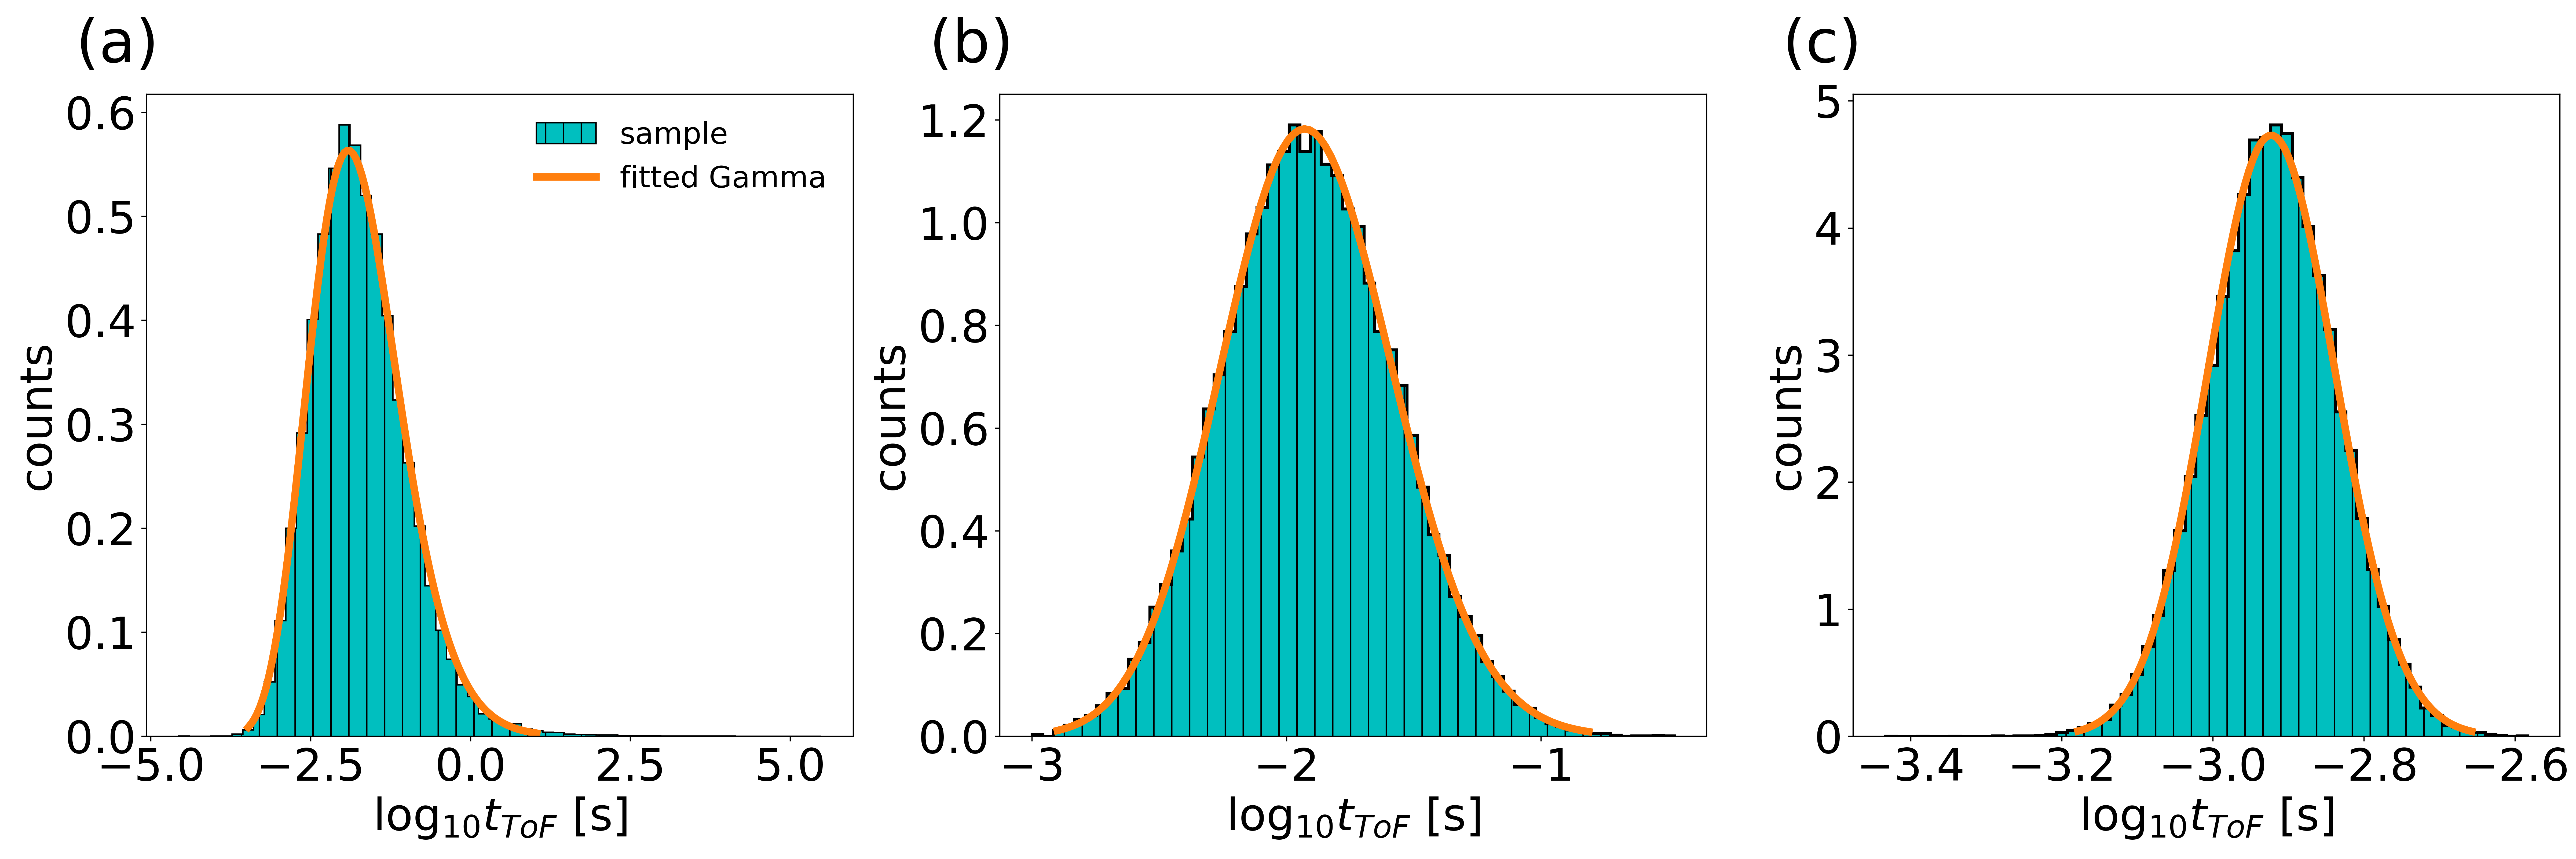
\includegraphics[width=0.9\textwidth]{figs/fig_mle.png}
    \caption{(a)The ToF distribution for 100000 samples where each $E_i$ is drawn from $N(\bar{E}_i,\sigma(E_i))$. The red curve is fitted to a gamma distribution. (b)The ToF distribution for 100000 samples where each $\lambda$ is drawn from $N(\bar{\lambda},\sigma(\lambda))$.(c)The ToF distribution for 100000 samples when each $J_{ij}$ is drawn from $N(\bar{J_{ij}},\sigma(J_{ij}))$.}
    \label{fig:ToFs}
\end{figure} 

This figure shows that ToF is more sensitive to change in $E_i$ and least sensitive to $J_{ij}$, even though from the scatter plots Fig.\ref{fig:scatterJ} the $J_{ij}$ has a very large magnitude deviation. 

The dataset of $\log_{10}(\text{ToF})$ can be well-fitted to a Gamma distribution. 
The statistical calculation has results:
\begin{itemize}
    \item When $E_i \in N(\bar{E_i},\sigma(E_i))$, the $\log_{10}(\text{ToF})$ has mean -1.73 and a standard deviation of 0.73.
    \item When $\lambda \in N(\bar{\lambda},\sigma(\lambda))$, the $\log_{10}(\text{ToF})$ has mean -1.91 and a standard deviation of 0.34.
    \item When $J_{ij} \in N(\bar{J_{ij}},\sigma(J_{ij}))$, the $\log_{10}(\text{ToF})$ has mean -2.92 and a standard deviation of 0.08.
\end{itemize}

When we use $E_i \in N(\bar{E_i},\sigma(E_i))$, $\lambda \in N(\bar{\lambda},\sigma(\lambda))$, $J_{ij} \in N(\bar{J_{ij}},\sigma(J_{ij}))$ at the same to perform the Monte Carlo sampling of ToF calculation, the ToF is shown in Fig.\ref{fig:ToFs2}. the $\log_{10}(\text{ToF})$ has mean -2.72 and a standard deviation of 0.80. To obtain a 90\% confidence level, then $-3.93 < \log_{10}(\text{ToF}) < -1.30$.
\begin{figure}
    \centering
    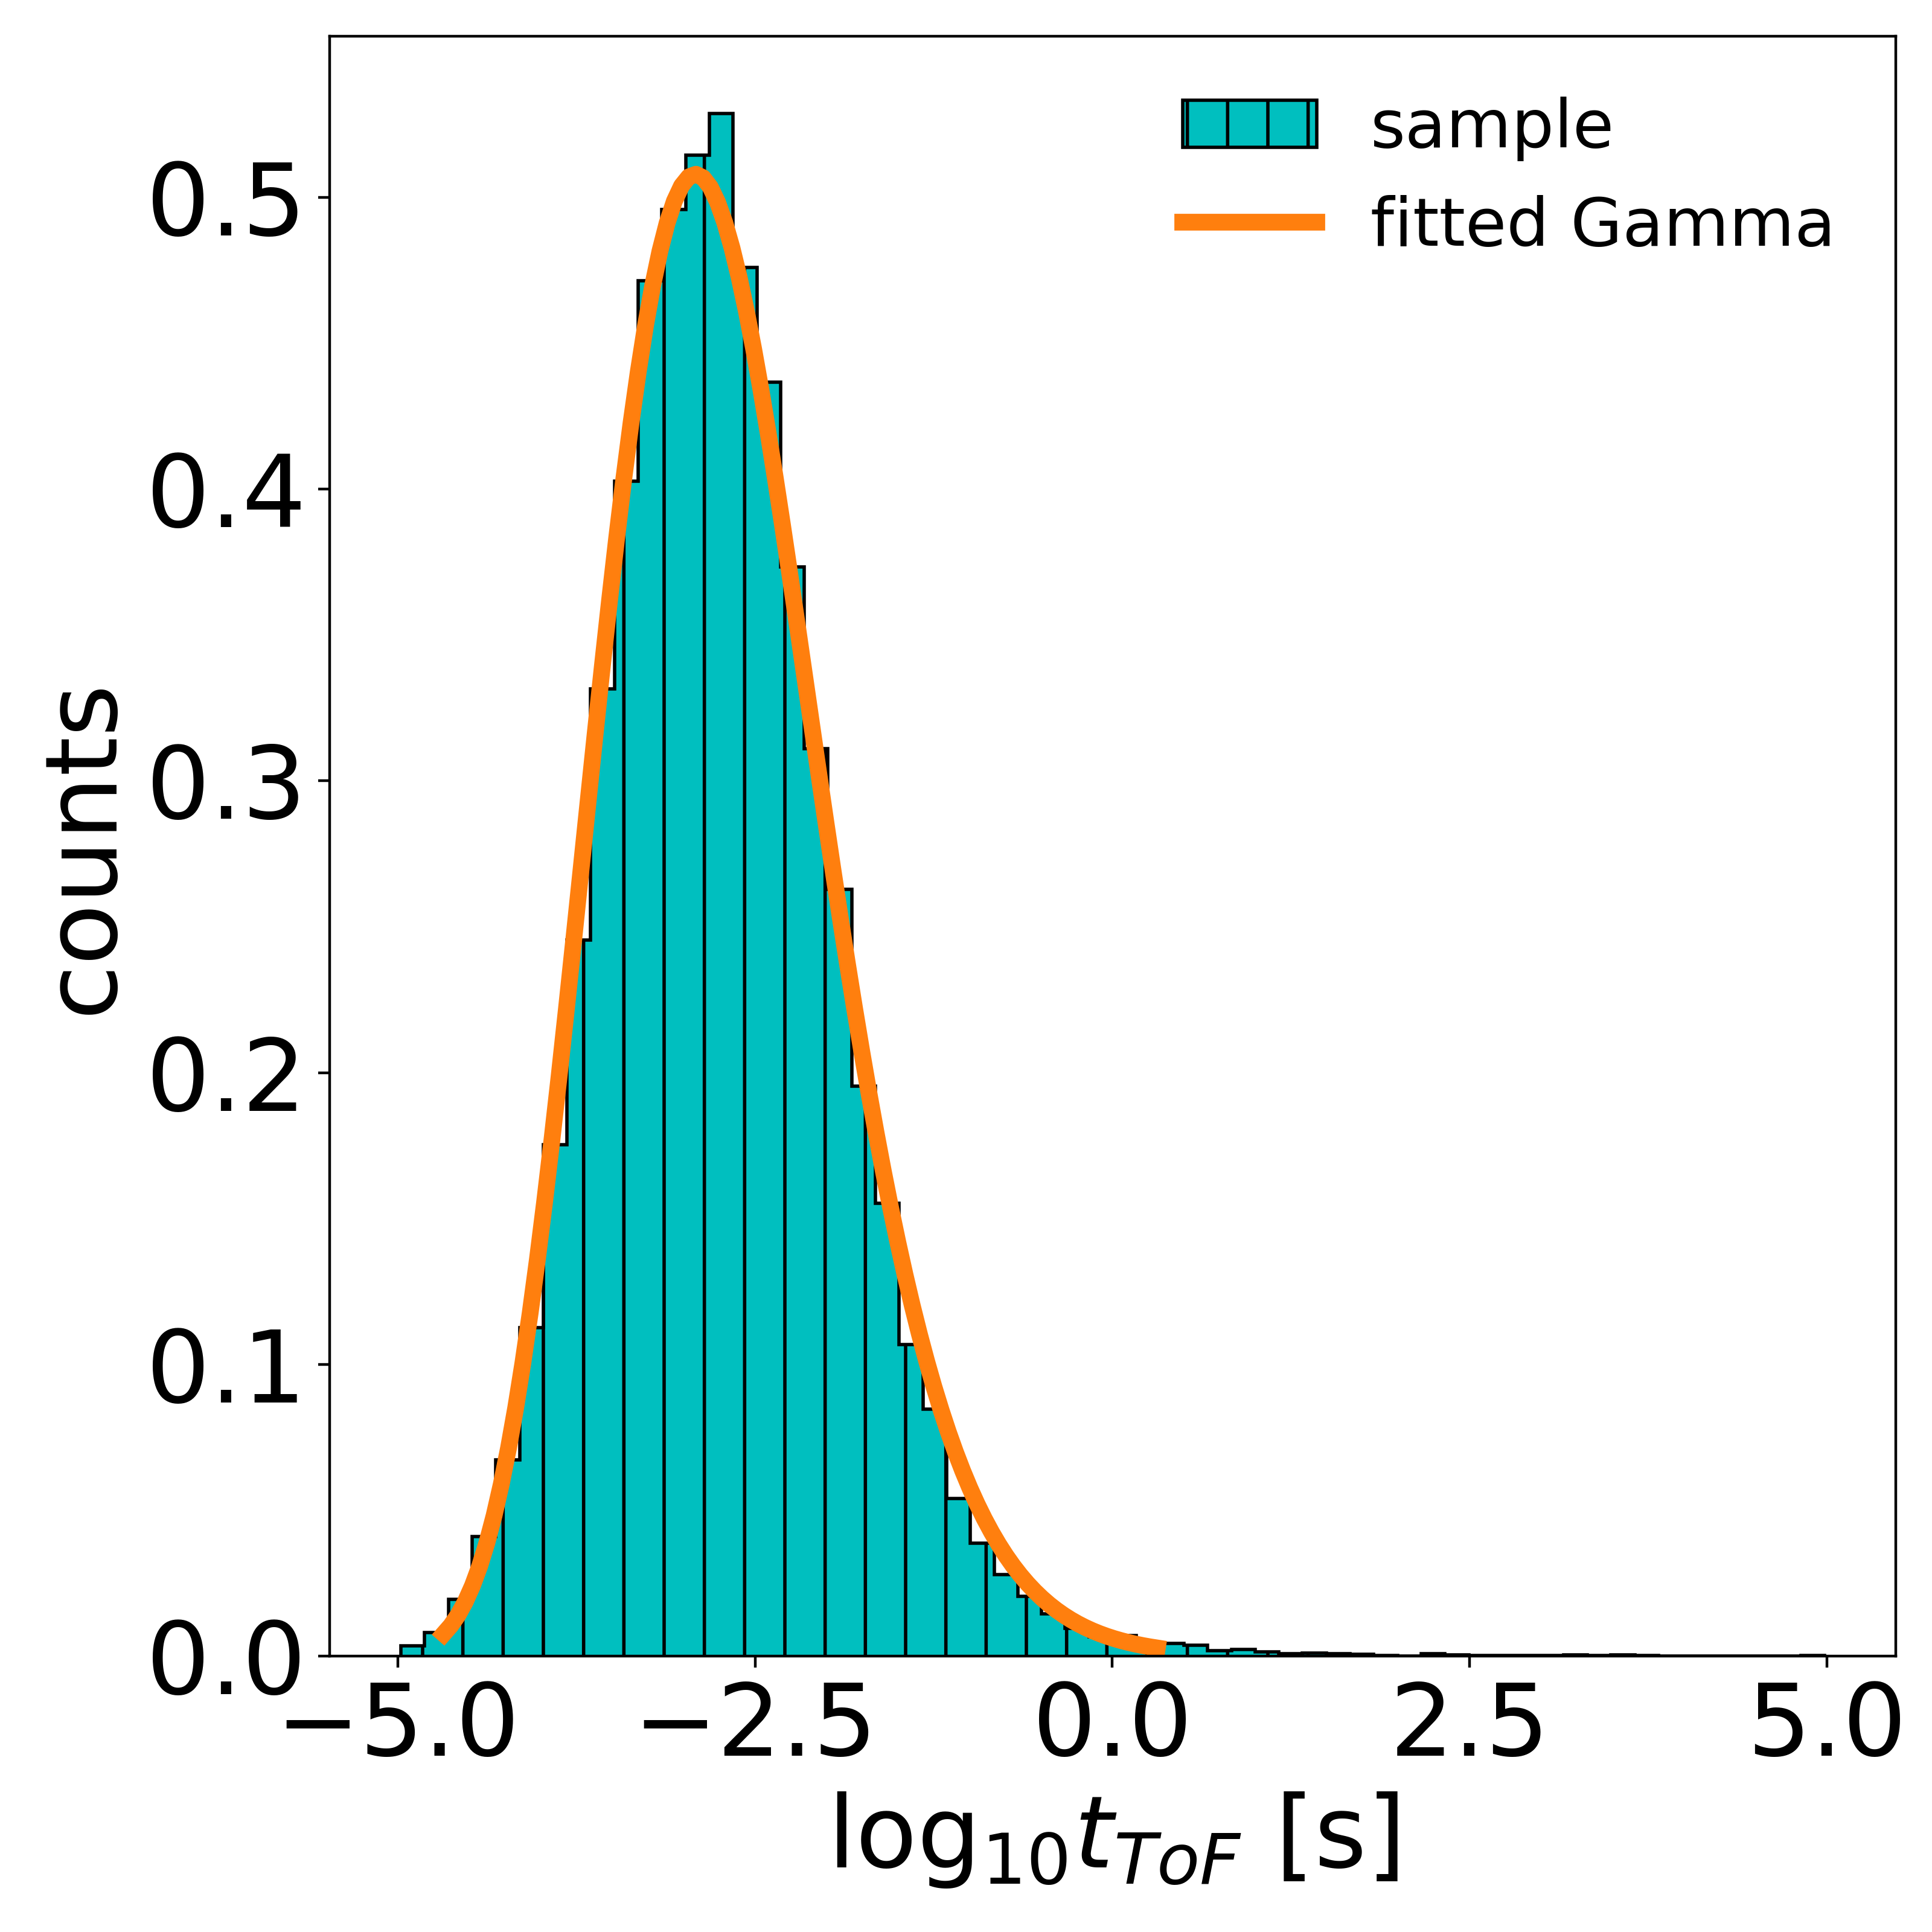
\includegraphics[width=0.6\textwidth]{figs/fig_mle2.png}
    \caption{The ToF distribution for 100000 samples where each $E_i$ is drawn from $N(\bar{E}_i,\sigma(E_i))$, $\lambda$ is drawn from $N(\bar{\lambda},\sigma(\lambda))$, and each $J_{ij}$ is drawn from $N(\bar{J_{ij}},\sigma(J_{ij}))$. The red curve is fitted to a gamma distribution.}
    \label{fig:ToFs2}
\end{figure} 

\section{Uncertainty in ToF}
Now we need to answer which ToF is accurate. 
Using the multiscale model to determine the ToF is a function $f: \mathbb{R}^d \rightarrow \mathbb{R}^+$, which maps the parameter vector $$\vec{x} = [ E_1,E_2,\cdots,E_N, R_1,R_2,\cdots,R_N,J_1,J_2,\cdots,J_{N_\text{pair}} ]$$ to a real value $\tau \in \mathbb{R}^+$.

Due to noise and approximation in the multiscale model, each element in $\vec{x}$ can be considered as an exact value plus an error term, for example $$E_1 = \hat{E}_1 + \epsilon_{E_1} $$
There is no prior knowledge about this error terms. 
Since the normal distribution inserts the least amount of prior knowledge into a model and encodes the maximum amount of uncertainty, we want to quantify the uncertainty when those error terms are normally distributed. 
\end{comment}


\end{document}